% **************************************************************************************************************
% A Classic Thesis Style
% An Homage to The Elements of Typographic Style
%
% Copyright (C) 2012 Andr\'e Miede http://www.miede.de
%
% If you like the style then I would appreciate a postcard. My address 
% can be found in the file ClassicThesis.pdf. A collection of the 
% postcards I received so far is available online at 
% http://postcards.miede.de
%
% License:
% This program is free software; you can redistribute it and/or modify
% it under the terms of the GNU General Public License as published by
% the Free Software Foundation; either version 2 of the License, or
% (at your option) any later version.
%
% This program is distributed in the hope that it will be useful,
% but WITHOUT ANY WARRANTY; without even the implied warranty of
% MERCHANTABILITY or FITNESS FOR A PARTICULAR PURPOSE.  See the
% GNU General Public License for more details.
%
% You should have received a copy of the GNU General Public License
% along with this program; see the file COPYING.  If not, write to
% the Free Software Foundation, Inc., 59 Temple Place - Suite 330,
% Boston, MA 02111-1307, USA.
%
% **************************************************************************************************************
% Note:
%    * You must not use "u etc. in strings/commands that will be spaced out (use \"u or real umlauts instead)
%    * New enumeration (small caps): \begin{aenumerate} \end{aenumerate}
%    * For margin notes: \marginpar or \graffito{}
%    * Do not use bold fonts in this style, it is designed around them
%    * Use tables as in the examples
%    * See classicthesis-preamble.sty for useful commands
% **************************************************************************************************************
% To Do:
%    * [high] Check this out: http://www.golatex.de/koma-script-warnung-in-verbindung-mit-listings-package-t2058.html
%    * [medium] mathbb in section-titles/chapter-titles => disappears somehow in headlines!!!
% **************************************************************************************************************
%TODO: openright?
\documentclass[ twoside,openany,titlepage,numbers=noenddot,headinclude,%
                footinclude=true,cleardoublepage=empty,abstractoff, % <--- obsolete, remove (todo)
                BCOR=5mm,paper=a4,fontsize=11pt,american,%
                draft]{scrreprt}

%********************************************************************
% Note: Make all your adjustments in here
%*******************************************************
\PassOptionsToPackage{utf8}{inputenc}
\usepackage{inputenc}
% ****************************************************************************************************
% classicthesis-config.tex
% formerly known as loadpackages.sty, classicthesis-ldpkg.sty, and classicthesis-preamble.sty
% Use it at the beginning of your ClassicThesis.tex, or as a LaTeX Preamble
% in your ClassicThesis.{tex,lyx} with \PassOptionsToPackage{utf8}{inputenc}
\usepackage{inputenc}
% ****************************************************************************************************
% classicthesis-config.tex
% formerly known as loadpackages.sty, classicthesis-ldpkg.sty, and classicthesis-preamble.sty
% Use it at the beginning of your ClassicThesis.tex, or as a LaTeX Preamble
% in your ClassicThesis.{tex,lyx} with \PassOptionsToPackage{utf8}{inputenc}
\usepackage{inputenc}
% ****************************************************************************************************
% classicthesis-config.tex
% formerly known as loadpackages.sty, classicthesis-ldpkg.sty, and classicthesis-preamble.sty
% Use it at the beginning of your ClassicThesis.tex, or as a LaTeX Preamble
% in your ClassicThesis.{tex,lyx} with \input{classicthesis-config}
% ****************************************************************************************************
% If you like the classicthesis, then I would appreciate a postcard.
% My address can be found in the file ClassicThesis.pdf. A collection
% of the postcards I received so far is available online at
% http://postcards.miede.de
% ****************************************************************************************************

% ****************************************************************************************************
% 1. Configure classicthesis for your needs here, e.g., remove "drafting" below
% in order to deactivate the time-stamp on the pages
% ****************************************************************************************************
\PassOptionsToPackage{eulerchapternumbers,listings,drafting,%
                 pdfspacing,%floatperchapter,%linedheaders,eulermath%
                 subfig,beramono}{classicthesis}
% ********************************************************************
% Available options for classicthesis.sty
% (see ClassicThesis.pdf for more information):
% drafting
% parts nochapters linedheaders
% eulerchapternumbers beramono eulermath pdfspacing minionprospacing
% tocaligned dottedtoc manychapters
% listings floatperchapter subfig
% ********************************************************************

% ********************************************************************
% Triggers for this config
% ********************************************************************
\usepackage{ifthen}
\newboolean{enable-backrefs} % enable backrefs in the bibliography
\setboolean{enable-backrefs}{false} % true false
% ****************************************************************************************************


\include{info}
% ********************************************************************
% Setup, finetuning, and useful commands
% ********************************************************************
\newlength{\abcd} % for ab..z string length calculation
\newcommand{\ie}{i.\,e.}
\newcommand{\Ie}{I.\,e.}
\newcommand{\eg}{e.\,g.}
\newcommand{\Eg}{E.\,g.}
\newcommand{\datasetRow}{\rowcolor{Moccasin}}
% ****************************************************************************************************


% ****************************************************************************************************
% 3. Loading some handy packages
% ****************************************************************************************************
% ********************************************************************
% Packages with options that might require adjustments
% ********************************************************************
\usepackage{etoolbox}
\newtoggle{EXTERNALPGF}
\toggletrue{EXTERNALPGF}
% \togglefalse{EXTERNALPGF}

\PassOptionsToPackage{american}{babel}   % change this to your language(s)
 \usepackage{babel}

% \PassOptionsToPackage{square,numbers}{natbib}
%  \usepackage{natbib}
\PassOptionsToPackage{style=ieee,sorting=nyt,backend=biber,defernumbers=true}{biblatex}
\usepackage{biblatex}
\addbibresource{strip.bib}

\PassOptionsToPackage{fleqn}{amsmath}        % math environments and more by the AMS
 \usepackage{amsmath}
 \usepackage{amssymb}
\usepackage{stmaryrd}
\PassOptionsToPackage{noautolanguage}{numprint}
\usepackage{numprint}
\npstyleenglish
\usepackage{geometry}
\usepackage{fancyvrb}
\PassOptionsToPackage{svgnames}{xcolor}
\usepackage{colortbl}
\usepackage{pgfplotstable}
\input{figure-params.tex}
% ********************************************************************
% General useful packages
% ********************************************************************
\PassOptionsToPackage{T1}{fontenc} % T2A for cyrillics
    \usepackage{fontenc}
\usepackage{textcomp} % fix warning with missing font shapes
\usepackage{scrhack} % fix warnings when using KOMA with listings package
\usepackage{mparhack} % get marginpar right
\usepackage{fixltx2e} % fixes some LaTeX stuff
\PassOptionsToPackage{printonlyused,smaller}{acronym}
    \usepackage{acronym} % nice macros for handling all acronyms in the thesis
%\renewcommand*{\acsfont}[1]{\textssc{#1}} % for MinionPro
\renewcommand{\bflabel}[1]{{#1}\hfill} % fix the list of acronyms
% ****************************************************************************************************


% ****************************************************************************************************
% 4. Setup floats: tables, (sub)figures, and captions
% ****************************************************************************************************
\usepackage{tabularx} % better tables
    \setlength{\extrarowheight}{3pt} % increase table row height
\newcommand{\tableheadline}[1]{\multicolumn{1}{c}{\spacedlowsmallcaps{#1}}}
\newcommand{\myfloatalign}{\centering} % to be used with each float for alignment
\usepackage{caption}
\captionsetup{format=hang,font=small}
\usepackage{subcaption}
% ****************************************************************************************************


% ****************************************************************************************************
% 5. Setup code listings
% ****************************************************************************************************
\usepackage{listings}
%\lstset{emph={trueIndex,root},emphstyle=\color{BlueViolet}}%\underbar} % for special keywords
\lstset{language=[LaTeX]Tex,%C++,
    keywordstyle=\color{RoyalBlue},%\bfseries,
    basicstyle=\small\ttfamily,
    %identifierstyle=\color{NavyBlue},
    commentstyle=\color{Green}\ttfamily,
    stringstyle=\rmfamily,
    numbers=none,%left,%
    numberstyle=\scriptsize,%\tiny
    stepnumber=5,
    numbersep=8pt,
    showstringspaces=false,
    breaklines=true,
    frameround=ftff,
    frame=single,
    belowcaptionskip=.75\baselineskip
    %frame=L
}
% ****************************************************************************************************


% ****************************************************************************************************
% 6. PDFLaTeX, hyperreferences and citation backreferences
% ****************************************************************************************************
% ********************************************************************
% Using PDFLaTeX
% ********************************************************************
\usepackage{varioref}
\PassOptionsToPackage{hyperfootnotes=false,pdfpagelabels}{hyperref}
    \usepackage{hyperref}  % backref linktocpage pagebackref
\pdfcompresslevel=8
\pdfadjustspacing=1
% \PassOptionsToPackage{pdftex}{graphicx}
    \usepackage{graphicx}
\graphicspath{{./gfx/}{./mkfigs/}}

% ********************************************************************
% Setup the style of the backrefs from the bibliography
% (translate the options to any language you use)
% ********************************************************************
\newcommand{\backrefnotcitedstring}{\relax}%(Not cited.)
\newcommand{\backrefcitedsinglestring}[1]{(Cited on page~#1.)}
\newcommand{\backrefcitedmultistring}[1]{(Cited on pages~#1.)}
\ifthenelse{\boolean{enable-backrefs}}%
{%
        \PassOptionsToPackage{hyperpageref}{backref}
        \usepackage{backref} % to be loaded after hyperref package
           \renewcommand{\backreftwosep}{ and~} % separate 2 pages
           \renewcommand{\backreflastsep}{, and~} % separate last of longer list
           \renewcommand*{\backref}[1]{}  % disable standard
           \renewcommand*{\backrefalt}[4]{% detailed backref
              \ifcase #1 %
                 \backrefnotcitedstring%
              \or%
                 \backrefcitedsinglestring{#2}%
              \else%
                 \backrefcitedmultistring{#2}%
              \fi}%
}{\relax}

% ********************************************************************
% Hyperreferences
% ********************************************************************
\hypersetup{%
    % draft,    % = no hyperlinking at all (useful in b/w printouts)
    colorlinks=true, linktocpage=true, pdfstartpage=3, pdfstartview=FitV,%
    % uncomment the following line if you want to have black links (e.g., for printing)
    %colorlinks=false, linktocpage=false, pdfborder={0 0 0}, pdfstartpage=3, pdfstartview=FitV,%
    breaklinks=true, pdfpagemode=UseNone, pageanchor=true, pdfpagemode=UseOutlines,%
    plainpages=false, bookmarksnumbered, bookmarksopen=true, bookmarksopenlevel=1,%
    hypertexnames=true, pdfhighlight=/O,%nesting=true,%frenchlinks,%
    urlcolor=webbrown, linkcolor=RoyalBlue, citecolor=webgreen, %pagecolor=RoyalBlue,%
    %urlcolor=Black, linkcolor=Black, citecolor=Black, %pagecolor=Black,%
    pdftitle={\myTitle},%
    pdfauthor={\textcopyright\ \myName, \myUni, \myFaculty},%
    pdfsubject={},%
    pdfkeywords={},%
    pdfcreator={pdfLaTeX},%
    pdfproducer={LaTeX with hyperref and classicthesis}%
}

% ********************************************************************
% Setup autoreferences
% ********************************************************************
% There are some issues regarding autorefnames
% http://www.ureader.de/msg/136221647.aspx
% http://www.tex.ac.uk/cgi-bin/texfaq2html?label=latexwords
% you have to redefine the makros for the
% language you use, e.g., american, ngerman
% (as chosen when loading babel/AtBeginDocument)
% ********************************************************************
\makeatletter
\@ifpackageloaded{babel}%
    {%
       \addto\extrasamerican{%
                    \renewcommand*{\figureautorefname}{Figure}%
                    \renewcommand*{\tableautorefname}{Table}%
                    \renewcommand*{\partautorefname}{Part}%
                    \renewcommand*{\chapterautorefname}{Chapter}%
                    \renewcommand*{\sectionautorefname}{Section}%
                    \renewcommand*{\subsectionautorefname}{Section}%
                    \renewcommand*{\subsubsectionautorefname}{Section}%
                }%
            % Fix to getting autorefs for subfigures right (thanks to Belinda Vogt for changing the definition)
            \providecommand{\subfigureautorefname}{\figureautorefname}%
    }{\relax}
\makeatother


% ****************************************************************************************************
% 7. Last calls before the bar closes
% ****************************************************************************************************
% ********************************************************************
% Development Stuff
% ********************************************************************
% \listfiles
%\PassOptionsToPackage{l2tabu,orthodox,abort}{nag}
%    \usepackage{nag}
%\PassOptionsToPackage{warning, all}{onlyamsmath}
%    \usepackage{onlyamsmath}

% ********************************************************************
% Last, but not least...
% ********************************************************************
\usepackage{classicthesis}
% \usepackage{arsclassica}
% ****************************************************************************************************


% ****************************************************************************************************
% 8. Further adjustments (experimental)
% ****************************************************************************************************
% ********************************************************************
% Changing the text area
% ********************************************************************
%\linespread{1.05} % a bit more for Palatino
%\areaset[current]{312pt}{761pt} % 686 (factor 2.2) + 33 head + 42 head \the\footskip
%\setlength{\marginparwidth}{7em}%
%\setlength{\marginparsep}{2em}%

% ********************************************************************
% Using different fonts
% ********************************************************************
%\usepackage[oldstylenums]{kpfonts} % oldstyle notextcomp
% \usepackage[osf]{libertine}
\usepackage{hfoldsty} % Computer Modern with osf
%\usepackage[light,condensed,math]{iwona}
%\renewcommand{\sfdefault}{iwona}
%\usepackage[urw-garamond]{mathdesign} <-- no osf support :-(
% ****************************************************************************************************
\include{common-config}
\usepackage[xindy,style=long,nolist]{glossaries}
\makeglossaries
\renewcommand{\glsnamefont}[1]{\spacedlowsmallcaps{#1}}
\input{glossary}

% ****************************************************************************************************
% If you like the classicthesis, then I would appreciate a postcard.
% My address can be found in the file ClassicThesis.pdf. A collection
% of the postcards I received so far is available online at
% http://postcards.miede.de
% ****************************************************************************************************

% ****************************************************************************************************
% 1. Configure classicthesis for your needs here, e.g., remove "drafting" below
% in order to deactivate the time-stamp on the pages
% ****************************************************************************************************
\PassOptionsToPackage{eulerchapternumbers,listings,drafting,%
                 pdfspacing,%floatperchapter,%linedheaders,eulermath%
                 subfig,beramono}{classicthesis}
% ********************************************************************
% Available options for classicthesis.sty
% (see ClassicThesis.pdf for more information):
% drafting
% parts nochapters linedheaders
% eulerchapternumbers beramono eulermath pdfspacing minionprospacing
% tocaligned dottedtoc manychapters
% listings floatperchapter subfig
% ********************************************************************

% ********************************************************************
% Triggers for this config
% ********************************************************************
\usepackage{ifthen}
\newboolean{enable-backrefs} % enable backrefs in the bibliography
\setboolean{enable-backrefs}{false} % true false
% ****************************************************************************************************


\usepackage{xspace} % to get the spacing after macros right
% ****************************************************************************************************
% 2. Personal data and user ad-hoc commands
% ****************************************************************************************************
\newcommand{\mySubtitle}{Where is Beverly Hills in your town?\xspace}
\newcommand{\myTitle}{Finding similar neighborhoods across cities by mining human urban activity\xspace}
\newcommand{\myDegree}{Master of Science\xspace}
\newcommand{\myName}{Géraud Le Falher\xspace}
\newcommand{\myProf}{Aristides Gionis\xspace}
\newcommand{\mySupervisor}{Michael Mathioudakis\xspace}
\newcommand{\myFaculty}{School of Science\xspace}
\newcommand{\myDepartment}{Department of Information and Computer Science\xspace}
\newcommand{\myUni}{Aalto University\xspace}
\newcommand{\myLocation}{Espoo, Finland\xspace}
\newcommand{\myTime}{August 2014\xspace}
\newcommand{\myVersion}{version 1.0\xspace}

% Thesis setup
\newcommand{\TITLE}{\myTitle}
\newcommand{\SUBTITLE}{\mySubtitle}
\newcommand{\DATE}{August 9, 2014}
\newcommand{\SUPERVISOR}{Professor \myProf}
\newcommand{\INSTRUCTOR}{\mySupervisor, PhD}
\newcommand{\PROFESSORSHIP}{Data Mining}
\newcommand{\PROFCODE}{T-61}
\newcommand{\KEYWORDS}{smart cities, metric learning, clustering, data mining,
foursquare, flickr, earth movers distance, geolocation, neighborhood, twitter,
urban computing}
\newcommand{\LANGUAGE}{English}
\newcommand{\AUTHOR}{\myName}

% ********************************************************************
% Setup, finetuning, and useful commands
% ********************************************************************
\newlength{\abcd} % for ab..z string length calculation
\newcommand{\ie}{i.\,e.}
\newcommand{\Ie}{I.\,e.}
\newcommand{\eg}{e.\,g.}
\newcommand{\Eg}{E.\,g.}
\newcommand{\datasetRow}{\rowcolor{Moccasin}}
% ****************************************************************************************************


% ****************************************************************************************************
% 3. Loading some handy packages
% ****************************************************************************************************
% ********************************************************************
% Packages with options that might require adjustments
% ********************************************************************
\usepackage{etoolbox}
\newtoggle{EXTERNALPGF}
\toggletrue{EXTERNALPGF}
% \togglefalse{EXTERNALPGF}

\PassOptionsToPackage{american}{babel}   % change this to your language(s)
 \usepackage{babel}

% \PassOptionsToPackage{square,numbers}{natbib}
%  \usepackage{natbib}
\PassOptionsToPackage{style=ieee,sorting=nyt,backend=biber,defernumbers=true}{biblatex}
\usepackage{biblatex}
\addbibresource{strip.bib}

\PassOptionsToPackage{fleqn}{amsmath}        % math environments and more by the AMS
 \usepackage{amsmath}
 \usepackage{amssymb}
\usepackage{stmaryrd}
\PassOptionsToPackage{noautolanguage}{numprint}
\usepackage{numprint}
\npstyleenglish
\usepackage{geometry}
\usepackage{fancyvrb}
\PassOptionsToPackage{svgnames}{xcolor}
\usepackage{colortbl}
\usepackage{pgfplotstable}
\usepackage{hfoldsty} % Computer Modern with osf
\usetikzlibrary{plotmarks}
\pgfplotsset{compat=newest,
    axis x line=bottom, axis y line=left,
    axis line style={Gray,line width=0.3pt},
	tick label style={font=\footnotesize},
	label style={font=\footnotesize},
	title style={font=\footnotesize},
	every axis title shift=0pt,
    title style={font=\footnotesize},
    legend style={font=\footnotesize,line width=0.15pt,cells={line width=0.3pt}},
    major grid style={line width=0.1pt, PapayaWhip}
}
\definecolor{ck1}{HTML}{1F77B4}
\definecolor{ck2}{HTML}{AEC7E8}
\definecolor{ck3}{HTML}{FF7F0E}
\definecolor{ck4}{HTML}{FFBB78}
\definecolor{ck5}{HTML}{2CA02C}
\definecolor{ck6}{HTML}{98DF8A}
\definecolor{ck7}{HTML}{D62728}
\definecolor{ck8}{HTML}{FF9896}
\definecolor{ck9}{HTML}{9467BD}
\definecolor{ck10}{HTML}{C5B0D5}
\definecolor{ck11}{HTML}{8C564B}
\definecolor{ck12}{HTML}{C49C94}
\definecolor{ck13}{HTML}{E377C2}
\definecolor{ck14}{HTML}{F7B6D2}
\definecolor{ck15}{HTML}{7F7F7F}
\definecolor{ck16}{HTML}{C7C7C7}
\definecolor{ck17}{HTML}{BCBD22}
\definecolor{ck18}{HTML}{DBDB8D}
\definecolor{ck19}{HTML}{17BECF}
\definecolor{ck20}{HTML}{9EDAE5}
\definecolor{cat1}{HTML}{E41A1C}
\definecolor{cat2}{HTML}{377EB8}
\definecolor{cat3}{HTML}{4DAF4A}
\definecolor{cat4}{HTML}{984EA3}
\definecolor{cat5}{HTML}{FF7F00}
\definecolor{cat6}{HTML}{FFFF33}
\definecolor{cat7}{HTML}{A65628}
\definecolor{cat8}{HTML}{F781BF}
\definecolor{cat9}{HTML}{888888}
\definecolor{pale}{HTML}{FCF9FC}

% ********************************************************************
% General useful packages
% ********************************************************************
\PassOptionsToPackage{T1}{fontenc} % T2A for cyrillics
    \usepackage{fontenc}
\usepackage{textcomp} % fix warning with missing font shapes
\usepackage{scrhack} % fix warnings when using KOMA with listings package
\usepackage{mparhack} % get marginpar right
\usepackage{fixltx2e} % fixes some LaTeX stuff
\PassOptionsToPackage{printonlyused,smaller}{acronym}
    \usepackage{acronym} % nice macros for handling all acronyms in the thesis
%\renewcommand*{\acsfont}[1]{\textssc{#1}} % for MinionPro
\renewcommand{\bflabel}[1]{{#1}\hfill} % fix the list of acronyms
% ****************************************************************************************************


% ****************************************************************************************************
% 4. Setup floats: tables, (sub)figures, and captions
% ****************************************************************************************************
\usepackage{tabularx} % better tables
    \setlength{\extrarowheight}{3pt} % increase table row height
\newcommand{\tableheadline}[1]{\multicolumn{1}{c}{\spacedlowsmallcaps{#1}}}
\newcommand{\myfloatalign}{\centering} % to be used with each float for alignment
\usepackage{caption}
\captionsetup{format=hang,font=small}
\usepackage{subcaption}
% ****************************************************************************************************


% ****************************************************************************************************
% 5. Setup code listings
% ****************************************************************************************************
\usepackage{listings}
%\lstset{emph={trueIndex,root},emphstyle=\color{BlueViolet}}%\underbar} % for special keywords
\lstset{language=[LaTeX]Tex,%C++,
    keywordstyle=\color{RoyalBlue},%\bfseries,
    basicstyle=\small\ttfamily,
    %identifierstyle=\color{NavyBlue},
    commentstyle=\color{Green}\ttfamily,
    stringstyle=\rmfamily,
    numbers=none,%left,%
    numberstyle=\scriptsize,%\tiny
    stepnumber=5,
    numbersep=8pt,
    showstringspaces=false,
    breaklines=true,
    frameround=ftff,
    frame=single,
    belowcaptionskip=.75\baselineskip
    %frame=L
}
% ****************************************************************************************************


% ****************************************************************************************************
% 6. PDFLaTeX, hyperreferences and citation backreferences
% ****************************************************************************************************
% ********************************************************************
% Using PDFLaTeX
% ********************************************************************
\usepackage{varioref}
\PassOptionsToPackage{hyperfootnotes=false,pdfpagelabels}{hyperref}
    \usepackage{hyperref}  % backref linktocpage pagebackref
\pdfcompresslevel=8
\pdfadjustspacing=1
% \PassOptionsToPackage{pdftex}{graphicx}
    \usepackage{graphicx}
\graphicspath{{./gfx/}{./mkfigs/}}

% ********************************************************************
% Setup the style of the backrefs from the bibliography
% (translate the options to any language you use)
% ********************************************************************
\newcommand{\backrefnotcitedstring}{\relax}%(Not cited.)
\newcommand{\backrefcitedsinglestring}[1]{(Cited on page~#1.)}
\newcommand{\backrefcitedmultistring}[1]{(Cited on pages~#1.)}
\ifthenelse{\boolean{enable-backrefs}}%
{%
        \PassOptionsToPackage{hyperpageref}{backref}
        \usepackage{backref} % to be loaded after hyperref package
           \renewcommand{\backreftwosep}{ and~} % separate 2 pages
           \renewcommand{\backreflastsep}{, and~} % separate last of longer list
           \renewcommand*{\backref}[1]{}  % disable standard
           \renewcommand*{\backrefalt}[4]{% detailed backref
              \ifcase #1 %
                 \backrefnotcitedstring%
              \or%
                 \backrefcitedsinglestring{#2}%
              \else%
                 \backrefcitedmultistring{#2}%
              \fi}%
}{\relax}

% ********************************************************************
% Hyperreferences
% ********************************************************************
\hypersetup{%
    % draft,    % = no hyperlinking at all (useful in b/w printouts)
    colorlinks=true, linktocpage=true, pdfstartpage=3, pdfstartview=FitV,%
    % uncomment the following line if you want to have black links (e.g., for printing)
    %colorlinks=false, linktocpage=false, pdfborder={0 0 0}, pdfstartpage=3, pdfstartview=FitV,%
    breaklinks=true, pdfpagemode=UseNone, pageanchor=true, pdfpagemode=UseOutlines,%
    plainpages=false, bookmarksnumbered, bookmarksopen=true, bookmarksopenlevel=1,%
    hypertexnames=true, pdfhighlight=/O,%nesting=true,%frenchlinks,%
    urlcolor=webbrown, linkcolor=RoyalBlue, citecolor=webgreen, %pagecolor=RoyalBlue,%
    %urlcolor=Black, linkcolor=Black, citecolor=Black, %pagecolor=Black,%
    pdftitle={\myTitle},%
    pdfauthor={\textcopyright\ \myName, \myUni, \myFaculty},%
    pdfsubject={},%
    pdfkeywords={},%
    pdfcreator={pdfLaTeX},%
    pdfproducer={LaTeX with hyperref and classicthesis}%
}

% ********************************************************************
% Setup autoreferences
% ********************************************************************
% There are some issues regarding autorefnames
% http://www.ureader.de/msg/136221647.aspx
% http://www.tex.ac.uk/cgi-bin/texfaq2html?label=latexwords
% you have to redefine the makros for the
% language you use, e.g., american, ngerman
% (as chosen when loading babel/AtBeginDocument)
% ********************************************************************
\makeatletter
\@ifpackageloaded{babel}%
    {%
       \addto\extrasamerican{%
                    \renewcommand*{\figureautorefname}{Figure}%
                    \renewcommand*{\tableautorefname}{Table}%
                    \renewcommand*{\partautorefname}{Part}%
                    \renewcommand*{\chapterautorefname}{Chapter}%
                    \renewcommand*{\sectionautorefname}{Section}%
                    \renewcommand*{\subsectionautorefname}{Section}%
                    \renewcommand*{\subsubsectionautorefname}{Section}%
                }%
            % Fix to getting autorefs for subfigures right (thanks to Belinda Vogt for changing the definition)
            \providecommand{\subfigureautorefname}{\figureautorefname}%
    }{\relax}
\makeatother


% ****************************************************************************************************
% 7. Last calls before the bar closes
% ****************************************************************************************************
% ********************************************************************
% Development Stuff
% ********************************************************************
% \listfiles
%\PassOptionsToPackage{l2tabu,orthodox,abort}{nag}
%    \usepackage{nag}
%\PassOptionsToPackage{warning, all}{onlyamsmath}
%    \usepackage{onlyamsmath}

% ********************************************************************
% Last, but not least...
% ********************************************************************
\usepackage{classicthesis}
% \usepackage{arsclassica}
% ****************************************************************************************************


% ****************************************************************************************************
% 8. Further adjustments (experimental)
% ****************************************************************************************************
% ********************************************************************
% Changing the text area
% ********************************************************************
%\linespread{1.05} % a bit more for Palatino
%\areaset[current]{312pt}{761pt} % 686 (factor 2.2) + 33 head + 42 head \the\footskip
%\setlength{\marginparwidth}{7em}%
%\setlength{\marginparsep}{2em}%

% ********************************************************************
% Using different fonts
% ********************************************************************
%\usepackage[oldstylenums]{kpfonts} % oldstyle notextcomp
% \usepackage[osf]{libertine}
\usepackage{hfoldsty} % Computer Modern with osf
%\usepackage[light,condensed,math]{iwona}
%\renewcommand{\sfdefault}{iwona}
%\usepackage[urw-garamond]{mathdesign} <-- no osf support :-(
% ****************************************************************************************************
\newcommand{\comment}[1]{\small\em #1 \\ \normalsize\normalfont}
\DeclareMathOperator*{\argmax}{argmax}
\DeclareMathOperator*{\argmin}{argmin}
\renewcommand{\equiv}{\Leftrightarrow}
\newcommand{\vnorm}[1]{\left|\left|#1\right|\right|}

\usepackage[xindy,style=long,nolist]{glossaries}
\makeglossaries
\renewcommand{\glsnamefont}[1]{\spacedlowsmallcaps{#1}}
% http://dickimaw-books.com/latex/thesis/html/makeglossaries.html
\newacronym[description={A social network where the main interaction consist
of sharing one's location, the most known example being
Foursquare}]{lbsn}{LBSN}{Location Based Social Network} 
\newacronym[description={}]{itml}{ITML}{Information Theoretic Metric Learning} 


% ****************************************************************************************************
% If you like the classicthesis, then I would appreciate a postcard.
% My address can be found in the file ClassicThesis.pdf. A collection
% of the postcards I received so far is available online at
% http://postcards.miede.de
% ****************************************************************************************************

% ****************************************************************************************************
% 1. Configure classicthesis for your needs here, e.g., remove "drafting" below
% in order to deactivate the time-stamp on the pages
% ****************************************************************************************************
\PassOptionsToPackage{eulerchapternumbers,listings,drafting,%
                 pdfspacing,%floatperchapter,%linedheaders,eulermath%
                 subfig,beramono}{classicthesis}
% ********************************************************************
% Available options for classicthesis.sty
% (see ClassicThesis.pdf for more information):
% drafting
% parts nochapters linedheaders
% eulerchapternumbers beramono eulermath pdfspacing minionprospacing
% tocaligned dottedtoc manychapters
% listings floatperchapter subfig
% ********************************************************************

% ********************************************************************
% Triggers for this config
% ********************************************************************
\usepackage{ifthen}
\newboolean{enable-backrefs} % enable backrefs in the bibliography
\setboolean{enable-backrefs}{false} % true false
% ****************************************************************************************************


\usepackage{xspace} % to get the spacing after macros right
% ****************************************************************************************************
% 2. Personal data and user ad-hoc commands
% ****************************************************************************************************
\newcommand{\mySubtitle}{Where is Beverly Hills in your town?\xspace}
\newcommand{\myTitle}{Finding similar neighborhoods across cities by mining human urban activity\xspace}
\newcommand{\myDegree}{Master of Science\xspace}
\newcommand{\myName}{Géraud Le Falher\xspace}
\newcommand{\myProf}{Aristides Gionis\xspace}
\newcommand{\mySupervisor}{Michael Mathioudakis\xspace}
\newcommand{\myFaculty}{School of Science\xspace}
\newcommand{\myDepartment}{Department of Information and Computer Science\xspace}
\newcommand{\myUni}{Aalto University\xspace}
\newcommand{\myLocation}{Espoo, Finland\xspace}
\newcommand{\myTime}{August 2014\xspace}
\newcommand{\myVersion}{version 1.0\xspace}

% Thesis setup
\newcommand{\TITLE}{\myTitle}
\newcommand{\SUBTITLE}{\mySubtitle}
\newcommand{\DATE}{August 9, 2014}
\newcommand{\SUPERVISOR}{Professor \myProf}
\newcommand{\INSTRUCTOR}{\mySupervisor, PhD}
\newcommand{\PROFESSORSHIP}{Data Mining}
\newcommand{\PROFCODE}{T-61}
\newcommand{\KEYWORDS}{smart cities, metric learning, clustering, data mining,
foursquare, flickr, earth movers distance, geolocation, neighborhood, twitter,
urban computing}
\newcommand{\LANGUAGE}{English}
\newcommand{\AUTHOR}{\myName}

% ********************************************************************
% Setup, finetuning, and useful commands
% ********************************************************************
\newlength{\abcd} % for ab..z string length calculation
\newcommand{\ie}{i.\,e.}
\newcommand{\Ie}{I.\,e.}
\newcommand{\eg}{e.\,g.}
\newcommand{\Eg}{E.\,g.}
\newcommand{\datasetRow}{\rowcolor{Moccasin}}
% ****************************************************************************************************


% ****************************************************************************************************
% 3. Loading some handy packages
% ****************************************************************************************************
% ********************************************************************
% Packages with options that might require adjustments
% ********************************************************************
\usepackage{etoolbox}
\newtoggle{EXTERNALPGF}
\toggletrue{EXTERNALPGF}
% \togglefalse{EXTERNALPGF}

\PassOptionsToPackage{american}{babel}   % change this to your language(s)
 \usepackage{babel}

% \PassOptionsToPackage{square,numbers}{natbib}
%  \usepackage{natbib}
\PassOptionsToPackage{style=ieee,sorting=nyt,backend=biber,defernumbers=true}{biblatex}
\usepackage{biblatex}
\addbibresource{strip.bib}

\PassOptionsToPackage{fleqn}{amsmath}        % math environments and more by the AMS
 \usepackage{amsmath}
 \usepackage{amssymb}
\usepackage{stmaryrd}
\PassOptionsToPackage{noautolanguage}{numprint}
\usepackage{numprint}
\npstyleenglish
\usepackage{geometry}
\usepackage{fancyvrb}
\PassOptionsToPackage{svgnames}{xcolor}
\usepackage{colortbl}
\usepackage{pgfplotstable}
\usepackage{hfoldsty} % Computer Modern with osf
\usetikzlibrary{plotmarks}
\pgfplotsset{compat=newest,
    axis x line=bottom, axis y line=left,
    axis line style={Gray,line width=0.3pt},
	tick label style={font=\footnotesize},
	label style={font=\footnotesize},
	title style={font=\footnotesize},
	every axis title shift=0pt,
    title style={font=\footnotesize},
    legend style={font=\footnotesize,line width=0.15pt,cells={line width=0.3pt}},
    major grid style={line width=0.1pt, PapayaWhip}
}
\definecolor{ck1}{HTML}{1F77B4}
\definecolor{ck2}{HTML}{AEC7E8}
\definecolor{ck3}{HTML}{FF7F0E}
\definecolor{ck4}{HTML}{FFBB78}
\definecolor{ck5}{HTML}{2CA02C}
\definecolor{ck6}{HTML}{98DF8A}
\definecolor{ck7}{HTML}{D62728}
\definecolor{ck8}{HTML}{FF9896}
\definecolor{ck9}{HTML}{9467BD}
\definecolor{ck10}{HTML}{C5B0D5}
\definecolor{ck11}{HTML}{8C564B}
\definecolor{ck12}{HTML}{C49C94}
\definecolor{ck13}{HTML}{E377C2}
\definecolor{ck14}{HTML}{F7B6D2}
\definecolor{ck15}{HTML}{7F7F7F}
\definecolor{ck16}{HTML}{C7C7C7}
\definecolor{ck17}{HTML}{BCBD22}
\definecolor{ck18}{HTML}{DBDB8D}
\definecolor{ck19}{HTML}{17BECF}
\definecolor{ck20}{HTML}{9EDAE5}
\definecolor{cat1}{HTML}{E41A1C}
\definecolor{cat2}{HTML}{377EB8}
\definecolor{cat3}{HTML}{4DAF4A}
\definecolor{cat4}{HTML}{984EA3}
\definecolor{cat5}{HTML}{FF7F00}
\definecolor{cat6}{HTML}{FFFF33}
\definecolor{cat7}{HTML}{A65628}
\definecolor{cat8}{HTML}{F781BF}
\definecolor{cat9}{HTML}{888888}
\definecolor{pale}{HTML}{FCF9FC}

% ********************************************************************
% General useful packages
% ********************************************************************
\PassOptionsToPackage{T1}{fontenc} % T2A for cyrillics
    \usepackage{fontenc}
\usepackage{textcomp} % fix warning with missing font shapes
\usepackage{scrhack} % fix warnings when using KOMA with listings package
\usepackage{mparhack} % get marginpar right
\usepackage{fixltx2e} % fixes some LaTeX stuff
\PassOptionsToPackage{printonlyused,smaller}{acronym}
    \usepackage{acronym} % nice macros for handling all acronyms in the thesis
%\renewcommand*{\acsfont}[1]{\textssc{#1}} % for MinionPro
\renewcommand{\bflabel}[1]{{#1}\hfill} % fix the list of acronyms
% ****************************************************************************************************


% ****************************************************************************************************
% 4. Setup floats: tables, (sub)figures, and captions
% ****************************************************************************************************
\usepackage{tabularx} % better tables
    \setlength{\extrarowheight}{3pt} % increase table row height
\newcommand{\tableheadline}[1]{\multicolumn{1}{c}{\spacedlowsmallcaps{#1}}}
\newcommand{\myfloatalign}{\centering} % to be used with each float for alignment
\usepackage{caption}
\captionsetup{format=hang,font=small}
\usepackage{subcaption}
% ****************************************************************************************************


% ****************************************************************************************************
% 5. Setup code listings
% ****************************************************************************************************
\usepackage{listings}
%\lstset{emph={trueIndex,root},emphstyle=\color{BlueViolet}}%\underbar} % for special keywords
\lstset{language=[LaTeX]Tex,%C++,
    keywordstyle=\color{RoyalBlue},%\bfseries,
    basicstyle=\small\ttfamily,
    %identifierstyle=\color{NavyBlue},
    commentstyle=\color{Green}\ttfamily,
    stringstyle=\rmfamily,
    numbers=none,%left,%
    numberstyle=\scriptsize,%\tiny
    stepnumber=5,
    numbersep=8pt,
    showstringspaces=false,
    breaklines=true,
    frameround=ftff,
    frame=single,
    belowcaptionskip=.75\baselineskip
    %frame=L
}
% ****************************************************************************************************


% ****************************************************************************************************
% 6. PDFLaTeX, hyperreferences and citation backreferences
% ****************************************************************************************************
% ********************************************************************
% Using PDFLaTeX
% ********************************************************************
\usepackage{varioref}
\PassOptionsToPackage{hyperfootnotes=false,pdfpagelabels}{hyperref}
    \usepackage{hyperref}  % backref linktocpage pagebackref
\pdfcompresslevel=8
\pdfadjustspacing=1
% \PassOptionsToPackage{pdftex}{graphicx}
    \usepackage{graphicx}
\graphicspath{{./gfx/}{./mkfigs/}}

% ********************************************************************
% Setup the style of the backrefs from the bibliography
% (translate the options to any language you use)
% ********************************************************************
\newcommand{\backrefnotcitedstring}{\relax}%(Not cited.)
\newcommand{\backrefcitedsinglestring}[1]{(Cited on page~#1.)}
\newcommand{\backrefcitedmultistring}[1]{(Cited on pages~#1.)}
\ifthenelse{\boolean{enable-backrefs}}%
{%
        \PassOptionsToPackage{hyperpageref}{backref}
        \usepackage{backref} % to be loaded after hyperref package
           \renewcommand{\backreftwosep}{ and~} % separate 2 pages
           \renewcommand{\backreflastsep}{, and~} % separate last of longer list
           \renewcommand*{\backref}[1]{}  % disable standard
           \renewcommand*{\backrefalt}[4]{% detailed backref
              \ifcase #1 %
                 \backrefnotcitedstring%
              \or%
                 \backrefcitedsinglestring{#2}%
              \else%
                 \backrefcitedmultistring{#2}%
              \fi}%
}{\relax}

% ********************************************************************
% Hyperreferences
% ********************************************************************
\hypersetup{%
    % draft,    % = no hyperlinking at all (useful in b/w printouts)
    colorlinks=true, linktocpage=true, pdfstartpage=3, pdfstartview=FitV,%
    % uncomment the following line if you want to have black links (e.g., for printing)
    %colorlinks=false, linktocpage=false, pdfborder={0 0 0}, pdfstartpage=3, pdfstartview=FitV,%
    breaklinks=true, pdfpagemode=UseNone, pageanchor=true, pdfpagemode=UseOutlines,%
    plainpages=false, bookmarksnumbered, bookmarksopen=true, bookmarksopenlevel=1,%
    hypertexnames=true, pdfhighlight=/O,%nesting=true,%frenchlinks,%
    urlcolor=webbrown, linkcolor=RoyalBlue, citecolor=webgreen, %pagecolor=RoyalBlue,%
    %urlcolor=Black, linkcolor=Black, citecolor=Black, %pagecolor=Black,%
    pdftitle={\myTitle},%
    pdfauthor={\textcopyright\ \myName, \myUni, \myFaculty},%
    pdfsubject={},%
    pdfkeywords={},%
    pdfcreator={pdfLaTeX},%
    pdfproducer={LaTeX with hyperref and classicthesis}%
}

% ********************************************************************
% Setup autoreferences
% ********************************************************************
% There are some issues regarding autorefnames
% http://www.ureader.de/msg/136221647.aspx
% http://www.tex.ac.uk/cgi-bin/texfaq2html?label=latexwords
% you have to redefine the makros for the
% language you use, e.g., american, ngerman
% (as chosen when loading babel/AtBeginDocument)
% ********************************************************************
\makeatletter
\@ifpackageloaded{babel}%
    {%
       \addto\extrasamerican{%
                    \renewcommand*{\figureautorefname}{Figure}%
                    \renewcommand*{\tableautorefname}{Table}%
                    \renewcommand*{\partautorefname}{Part}%
                    \renewcommand*{\chapterautorefname}{Chapter}%
                    \renewcommand*{\sectionautorefname}{Section}%
                    \renewcommand*{\subsectionautorefname}{Section}%
                    \renewcommand*{\subsubsectionautorefname}{Section}%
                }%
            % Fix to getting autorefs for subfigures right (thanks to Belinda Vogt for changing the definition)
            \providecommand{\subfigureautorefname}{\figureautorefname}%
    }{\relax}
\makeatother


% ****************************************************************************************************
% 7. Last calls before the bar closes
% ****************************************************************************************************
% ********************************************************************
% Development Stuff
% ********************************************************************
% \listfiles
%\PassOptionsToPackage{l2tabu,orthodox,abort}{nag}
%    \usepackage{nag}
%\PassOptionsToPackage{warning, all}{onlyamsmath}
%    \usepackage{onlyamsmath}

% ********************************************************************
% Last, but not least...
% ********************************************************************
\usepackage{classicthesis}
% \usepackage{arsclassica}
% ****************************************************************************************************


% ****************************************************************************************************
% 8. Further adjustments (experimental)
% ****************************************************************************************************
% ********************************************************************
% Changing the text area
% ********************************************************************
%\linespread{1.05} % a bit more for Palatino
%\areaset[current]{312pt}{761pt} % 686 (factor 2.2) + 33 head + 42 head \the\footskip
%\setlength{\marginparwidth}{7em}%
%\setlength{\marginparsep}{2em}%

% ********************************************************************
% Using different fonts
% ********************************************************************
%\usepackage[oldstylenums]{kpfonts} % oldstyle notextcomp
% \usepackage[osf]{libertine}
\usepackage{hfoldsty} % Computer Modern with osf
%\usepackage[light,condensed,math]{iwona}
%\renewcommand{\sfdefault}{iwona}
%\usepackage[urw-garamond]{mathdesign} <-- no osf support :-(
% ****************************************************************************************************
\newcommand{\comment}[1]{\small\em #1 \\ \normalsize\normalfont}
\DeclareMathOperator*{\argmax}{argmax}
\DeclareMathOperator*{\argmin}{argmin}
\renewcommand{\equiv}{\Leftrightarrow}
\newcommand{\vnorm}[1]{\left|\left|#1\right|\right|}

\usepackage[xindy,style=long,nolist]{glossaries}
\makeglossaries
\renewcommand{\glsnamefont}[1]{\spacedlowsmallcaps{#1}}
% http://dickimaw-books.com/latex/thesis/html/makeglossaries.html
\newacronym[description={A social network where the main interaction consist
of sharing one's location, the most known example being
Foursquare}]{lbsn}{LBSN}{Location Based Social Network} 
\newacronym[description={}]{itml}{ITML}{Information Theoretic Metric Learning} 



%********************************************************************
% Hyphenation
%*******************************************************
%\hyphenation{put special hyphenation here}

% ********************************************************************
% GO!GO!GO! MOVE IT!
%*******************************************************
\begin{document}
% \frenchspacing
\raggedbottom
\selectlanguage{american}
%\renewcommand*{\bibname}{new name}
%\setbibpreamble{}
\pagenumbering{roman}
\pagestyle{plain}
%********************************************************************
% Frontmatter
%*******************************************************
% %*******************************************************
% Titlepage
%*******************************************************
\begin{titlepage}
	% if you want the titlepage to be centered, uncomment and fine-tune the line below (KOMA classes environment)
	\begin{addmargin}[-1cm]{-3cm}
    \begin{center}
        \large  

        \hfill

        \vfill

        \begingroup
            \color{Maroon}
	    \spacedallcaps{\myTitle} \\ \medskip
	    \mySubtitle \\ \medskip   
        \endgroup

	\vspace{2\baselineskip}
\begin{minipage}{0.4\textwidth}
\begin{flushleft} \large
\emph{Author:}\\
Géraud Le Falher\\
% {\footnotesize\url{geraud.lefalher@aalto.fi}}
\end{flushleft}
\end{minipage}
~
\begin{minipage}{0.4\textwidth}
\begin{flushright} \large
\emph{Supervisors:}\\
\myProf\\%[\baselineskip]
	% {\footnotesize\url{aristides.gionis@aalto.fi}}
\mySupervisor
	% {\footnotesize\url{michael.mathioudakis@hiit.fi}}
\end{flushright}
\end{minipage}
        % \spacedlowsmallcaps{Géraud Le Falher}
		% \myName{}

        \vfill

        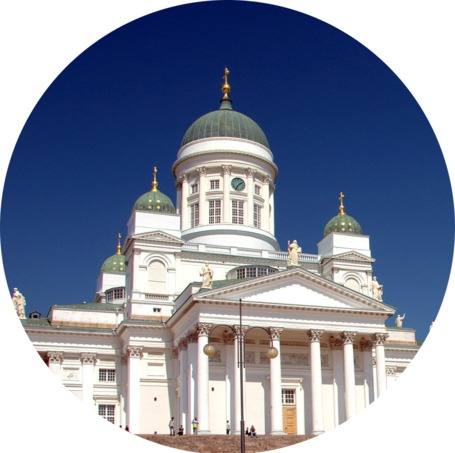
\includegraphics[width=0.4\textwidth]{gfx/helsinki} \quad
	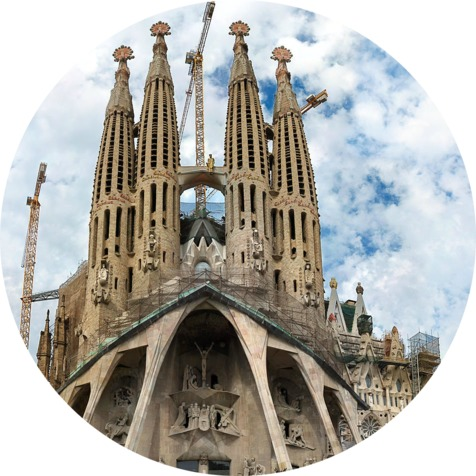
\includegraphics[width=0.4\textwidth]{gfx/barca.jpg}
	\vspace{3\baselineskip}
        \vfill

        \myDegree \\
        \myDepartment \\                            
        \myFaculty \\
        \myUni \\ \bigskip

        % \myTime\ -- \myVersion

        \vfill                      

    \end{center}  
  \end{addmargin}       
\end{titlepage}   

% \thispagestyle{empty}

\hfill

\vfill

\noindent\myName: \textit{\myTitle,} \mySubtitle, \myDegree, 
\textcopyright\ \myTime

\bigskip

\noindent\spacedlowsmallcaps{Supervisors}: \\
\myProf \\
\mySupervisor

\medskip

\noindent\spacedlowsmallcaps{Location}: \\
\myLocation
%
%\medskip
%
%\noindent\spacedlowsmallcaps{Time Frame}: \\
%\myTime

% \cleardoublepage%*******************************************************
% Dedication
%*******************************************************
\thispagestyle{empty}
%\phantomsection 
\refstepcounter{dummy}
\pdfbookmark[1]{Dedication}{Dedication}

\vspace*{3cm}


\begin{center}
	\emph{to the one above the stars.} \\ \smallskip
    1950\,--\,2009
\end{center}

% \cleardoublepage\pdfbookmark[1]{Abstract}{Abstract}
\begingroup
\let\clearpage\relax

\chapter*{Abstract}

We propose a method to match similar neighborhoods across different cities.
That is, we give ourselves a measure of similarity between urban regions, as
well as one region in one city. Our goal is to find the region in some other
cities which minimize the distance with the query region. Furthermore, we
seek to do it effienctly, as it is prohivitive to evaluate the distance of
all possible regions.

First, we collect trace of activities in 20 European and American cities from
location aware social platforms \fs{} and \flickr{}. A thorough exploration of
this dataset leads us to describe individual venues by relevant features
including their aggregate activity across time, their visitors and overall
popularity, and the typology of their surrounding.  Then we learned several
measures of venue similarity in a semi-supervised setting and evaluate their
performance on two information retrieval tasks.  After gathering human ground
truth about neighborhoods, we evaluate different metrics between sets of
venues and find out that earth movers distance is the best suited at assessing
neighborhood similarity. Finally, we address the computational efficiency
problem of finding the most similar neighborhood given a query. We devise a
heuristic search strategy and show that it provides results of comparable
quality while being order of magnitude faster. This work has application in
touristic recommendation and urban planning, as it provides a similarity
measure between urban areas.

\endgroup 
\vfill

%\cleardoublepage%*******************************************************
% Acknowledgments
%*******************************************************
\pdfbookmark[1]{Acknowledgments}{acknowledgments}

\begin{flushright}{\slshape    
		I can feel it in my bones \\
		So much left unknown \\
		We continue to grow old \\
		At least I found my gold
    } \\ \medskip
    --- \emph{Gold}, Vinyl Theathre\footnote{From their album of the same
	    name: \href{https://youtu.be/y_hSArYE4kI?t=2m45s}%
	    {\url{youtu.be/y_hSArYE4kI}}.}
\end{flushright}

\bigskip

\begingroup
\let\clearpage\relax
\let\cleardoublepage\relax
\let\cleardoublepage\relax
\chapter*{Acknowledgments}

I am greatly indebted to many people. First to my supervisor, Prof.\@ \myProf,
for suggesting me this topic, providing me thorough and kind guidance for more
than six months, and for compensating my usual lack of enthusiasm with his.
Coming second only by alphabetical order, I also want to offer my gratitude to
my advisor, Dr.\@ \mySupervisor for his help and his fine remarks concerning my
writing. This research wad conducted while I was part of the
Data Mining Group\footnote{\href{http://research.ics.aalto.fi/dmg/}%
{\url{research.ics.aalto.fi/dmg/}}} and I am thankful for having met such
nice and bright people (and for having eaten many different kinds of cake
during the meetings). Actually, I may as well thank all the people I have
worked with at \myUni, because it was a real pleasure. Even more broadly, this
time in Finland was a delight, made possible by the impressive, pristine nature
as as much by the kindness of people living there.

In addition to these talented and supportive people, this work would not have
been possible if not for many great open-source softwares. Yet because it would
feel weird to thanks them in the same place, I relegate them in \autoref{chap:ack}.

On a personal level, I would first like to thank the members of my family for
their unconditional support. I have also heavily relied on friends for their
knowledge on Paris; yet neither Camille Autran, Oliver Braud nor Aloïs Guillopé
have ever expressed any irritation (at least openly).  As I am finishing the
redaction of this manuscript, I have to acknowledge that, however frequent and
unexpected, the interruptions of Kiran Garimella were probably beneficial in
the long term. Finally, the outcome would certainly have been different without
the influence of Sanja Šćepanović; both objectively---for giving me the Twitter
API key used to collect my dataset--- and subjectively---for so many reasons that
it would be pointless to try to condense them in a few sentences.

\endgroup

\pagestyle{scrheadings}
% \cleardoublepage%*******************************************************
% Table of Contents
%*******************************************************
%\phantomsection
\refstepcounter{dummy}
\pdfbookmark[1]{\contentsname}{tableofcontents}
\setcounter{tocdepth}{2} % <-- 2 includes up to subsections in the ToC
\setcounter{secnumdepth}{3} % <-- 3 numbers up to subsubsections
\manualmark
\markboth{\spacedlowsmallcaps{\contentsname}}{\spacedlowsmallcaps{\contentsname}}
\tableofcontents 
\automark[section]{chapter}
\renewcommand{\chaptermark}[1]{\markboth{\spacedlowsmallcaps{#1}}{\spacedlowsmallcaps{#1}}}
\renewcommand{\sectionmark}[1]{\markright{\thesection\enspace\spacedlowsmallcaps{#1}}}
%*******************************************************
% List of Figures and of the Tables
%*******************************************************
\clearpage

\begingroup 
    \let\clearpage\relax
    \let\cleardoublepage\relax
    \let\cleardoublepage\relax
    %*******************************************************
    % List of Figures
    %*******************************************************    
    %\phantomsection 
    \refstepcounter{dummy}
    \setcounter{lofdepth}{2}
    %\addcontentsline{toc}{chapter}{\listfigurename}
    \pdfbookmark[1]{\listfigurename}{lof}
    \listoffigures

    \vspace*{8ex}

    %*******************************************************
    % List of Tables
    %*******************************************************
    %\phantomsection 
    \refstepcounter{dummy}
    %\addcontentsline{toc}{chapter}{\listtablename}
    \pdfbookmark[1]{\listtablename}{lot}
    \listoftables
        
    \vspace*{8ex}
%   \newpage
    
    %*******************************************************
    % List of Listings
    %*******************************************************      
	  %\phantomsection 
    % \refstepcounter{dummy}
    %\addcontentsline{toc}{chapter}{\lstlistlistingname}
    % \pdfbookmark[1]{\lstlistlistingname}{lol}
    % \lstlistoflistings
    %
    % \vspace*{8ex}
       
    %*******************************************************
    % Acronyms
    %*******************************************************
    %\phantomsection 
    \refstepcounter{dummy}
    \pdfbookmark[1]{Acronyms}{acronyms}
    \markboth{\spacedlowsmallcaps{Acronyms}}{\spacedlowsmallcaps{Acronyms}}
    \printglossary
\endgroup

\cleardoublepage

%********************************************************************
% Mainmatter
%*******************************************************
\pagenumbering{arabic}
%\setcounter{page}{90}
% use \cleardoublepage here to avoid problems with pdfbookmark
%\cleardoublepage
% \section{Motivation}
\label{sec:motivation}

More and more people are living in cities\footnote{According to an
\href{http://esa.un.org/unup/pdf/WUP2011_Highlights.pdf}{UN report}
\autocite{UNreport12}, \enquote{the population living in urban areas is
projected to [pass] from 3.6 billion in 2011 to 6.3 billion in 2050.}}. This
simple observation leads to two questions: how to help urban dwellers make
informed everyday decisions and how to understand these large and complex
systems. Fortunately, now is a good time to tackle these issues. Indeed, thanks
to social networks and mobile devices, we know where and when people are
active within cities \autocite{SpatialComputing12}. We seize this opportunity
to devise a similarity measure between urban areas. First we motivate the
need for such a measure through a typical use case:

\begin{quote}
Let us say you have lived in a city for the last years. During this time,
you have acquired urban knowledge that you can leverage to find relevant
locations where to perform various tasks. In simpler words, whether you want
to buy milk, listen to loud music or exhibit your athletic skills, you know
where to go. Yet life is full of surprises and you may be spending a few
days in a new town. Fair enough, but you do not want to renounce to your
wide range of outside activities. This is where our application comes in
handy. You select a location or an area in your familiar city and it shows
you a place or a zone sharing similar characteristics in your surroundings.
Thus you can boldly venture into distant shores, reassured that a part of
your home will always travel with you.
\end{quote}

% This short illustration gives an intuitive definition of the problem we are
% trying to solve. Namely, a user picks a small part of a city and we represent
% it by a bag of all venues it contains. These venues are associated with some
% features and we want to find, efficiently, a set of venues that shares similar
% characteristics. Yet for this result to be meaningful, we add the constraint
% that the venues must delineate a neighborhood, that is a small and compact
% subset of the whole city.

As this short illustration demonstrates, our problem has applications to
recommending locations in a city.
But it is also applicable in the analysis of cities and urban planning. For
instance, when applied to the neighborhoods of one city, our techniques allow
to identify neighborhoods that are similar to each other, and thus can help us
understand what is going on in each area, what are the hubs of different
activities, how citizens are experiencing the city, and how they are utilizing
its resources. 

\section{Problem definition}
\label{sec:problem}

Let us define formally this problem. We have a set of cities $\mathcal{C} =
\{c_1, c_2, \ldots, c_n\}$, each of them defined by a enclosing rectangle
$R_{c_i} \subseteq \mathbb{R}^2$. Furthermore, each city $c_i$ contains a
subset $V_{c_i} \subseteq \mathcal{V}$, where $\mathcal{V}$ is a set of
\emph{venues}. A \emph{venue} is an uniquely identified location that can be
visited by individuals. It includes for instance restaurants, shops, airports,
monuments and parks. Finally, each city $c_i$ is described by another subset
$I_{c_i} \subseteq \mathcal{I}$, where $\mathcal{I}$ is a set of \emph{items}.
These \emph{items} are user contributed discrete points in space and time that
can have additional attributes. Here, we exploit Flickr photos (with tags) and
Foursquare check-ins as type of item\footnote{But this definition can be
    extended to other kind of data. For instance, a tweet is a point in time
    and space (along with the sentiment it conveys). We can also consider
    noise and pollution measurements, the number of cars crossing a given
    intersection during a one minute window, Yelp reviews, etc. Stretching the
    concept, we could collect anonymized customer receipts from grocery shops.
    The attributes will then be the proportion in which different kind of
    goods are consumed. Indeed, even for two shops of the same company in the
    same city, it would give information about the neighboring population.}.
Items are associated with venues, either directly, like check-ins, or
indirectly, like photos. In the latter case, the relationship between venues
and items is based on spatial distance.

By combining venues own characteristics and their associated items, we want to
devise a similarity measure over the venues $\mathcal{V}$, namely $\delta:
\mathcal{V}^2 \rightarrow \llbracket 0, 1 \rrbracket $. This provides a
building block for another measure of similarity between two spatial regions.
More precisely, after choosing a home city $c_h$ and a target city
$c_t$\footnote{$t$ can also stand for travel or tourist.}, we want to
construct $\delta': R_{c_h} \times R_{c_t} \rightarrow \llbracket 0, 1 \rrbracket$.
These two functions answer the following queries:

\begin{enumerate}
\item When users pick a venue $v$ in their home city, find the venue in the
	target town that is the most similar to it. Formally, we compute
	$\argmax_{v' \in V_{c_t}} \delta(v, v')$.\label{q:point}
\item Instead of a single venue, users ask for a larger area $r$, for instance
	covering a neighborhood\footnote{or any other meaningful subdivision.}
	from their home city. In that case we also return an area:
	$\argmax_{r' \subseteq V_{c_t}} \delta'(r, r')$.\label{q:space}
\end{enumerate}


% \subsection*{Setup}
\comment{another way to say it:\\
We have two cities, $C_1$ and $C_2$. In each of them lie objects of different
kind (in our case: photos, check-ins and venues). These objects have a
position in $\mathbb{R}^2$, along with other attributes like time, tags,
category or number of visitors.

% \subsection*{Goal}
As an input, we are given a polygonal region $R$ contained in $C_1$. The
desired output is the region $R'$ in $C_2$ that is closest to $R$ according
to the metric $\delta_{\theta}$.
}

% \subsection*{Problem}

A region is represented by the $e'$ main objects it contains (the venues).
Each of these venues is in turn described by $d$ numerical features. In
addition, each region have a set of $g$ global features that are not
associated with any specific objects. Thus a region $R$ is fully characterized
by
\begin{align*}
	\phi \colon \mathcal{R} &\to
	\mathbb{R}^{e'\times d} \times \mathbb{R}^g = \mathcal{F} \\
	R &\mapsto (X, x)
\end{align*}

Inside $\mathcal{F}$, two regions can be compared using the
$\theta$-parametrized distance
\begin{align*}
	\delta_{\theta} \colon &\mathcal{F} \times \mathcal{F} \to
	\mathbb{R}^+ \\
	&(X, x) , (X', x') \mapsto d_{R,R'}
\end{align*}

and our our objective is fulfilled by computing, for a given $R \in
\mathcal{R}(C_1)$
\begin{equation}
	\argmin_{R' \in \mathcal{R}(C_2)}\; \delta_{\theta}
	\left(\phi(R), \phi(R')\right)
	\label{e:onetheta}
\end{equation}

More precisely, $\delta_{\theta}$ is defined as follow. Let $X_i$ (respectively
$X'_i$) be the $i$\textsuperscript{th} column of $X$ ($X'$), $P_i$ ($Q_i$) the
associated distribution, $D_{\mathrm{KL}}(P \parallel Q) = \sum_j
P(j)\ln\left(\frac{P(j)}{Q(j)}\right)$ the Kullback--Leibler divergence
between $P$ and $Q$ and $ \mathrm{JSD}(P \parallel Q)=
\frac{1}{2}D_{\mathrm{KL}}(P \parallel M)+\frac{1}{2}D_{\mathrm{KL}}(Q
\parallel M)$ their Jensen--Shannon divergence \autocite{JensenShannon03},
where $M=\frac{1}{2}(P+Q)$. Then
\[
	\delta_{\theta} \left(\phi(R), \phi(R')\right) = \sum_{i=1}^d
	\theta_i \mathrm{JSD}(P_i \parallel Q_i) + \vnorm{x - x'}
\]

\subsection*{Additional considerations}
\subsubsection*{Point Pattern Matching}

A more refined answer would acknowledge that not all regions can be compared in
the same way and thus solve
\begin{equation}
    \argmin_{\theta ,\, R' \in \mathcal{R}(C_2)}\; \delta_{\theta}
    \left(\phi(R), \phi(R')\right) + cost(\theta)
    \label{e:manythetas}
\end{equation}
where the regularisation of $\theta$ ensures that there is still a common
ground in the way similarity is computed.

\eqref{e:manythetas} can be casted as a \emph{Point Pattern
Matching}\footnote{Also known as \emph{Point set registration}.} problem.
Following \textcite{PointPatternMatching08}, let $P$ be the $e'$ points of
$\mathbb{R}^d$ that make up $R$, and let $T$ be the $n$ points of
$\mathbb{R}^d$ lying in $C_2$. The problem asks whether there is a subset $I
\subseteq T$ such that $\delta_{\theta}\left(P, I\right) \leq \epsilon$. In
this case, $\theta$ represents a linear transformation applied to $P$. And
instead of explicit regularisation, it can only be drawn from a fixed class of
transformations. Another constraint is that $I$ must be restricted to subsets
of venues that indeed form neighborhood.

\subsubsection*{The choice of $\delta$}

Here are presented some design alternatives for $\delta$ and why the current
choice was made.

\begin{itemize}
    \item First, weighting venues, either explicitly or, more likely,
        implicitly (for instance by their relative popularity in the region)
        will provide more flexibility. Especially, a fixed fraction of venues
        may have zero weight because we consider they don't really belong to a
        given neighborhood.
    \item There are different distances between two point sets. For instance,
        the bottleneck distance \autocite{Bottleneck96} (the smallest distance
        between pairs of farthest point), the sum of the distance of each
        point to its closest neighbor, or the Hausdorff distance (the largest
        distance between pairs of closest point) and its variation
        \autocite{ModifiedHausdorff94}. From what I have seen, these measures
        have been used mostly in 2 or 3 dimensional space.  Thus it would be
        interesting to see how they behave in higher dimension.  Especially
        since linear transformations in $\mathbb{R}^{31}$ are not very
        intuitive.
    \item Instead of using euclidean distance to compare global feature, some
	    histogram distance \autocite{HistogramDistance02} may be more suited,
        especially to compare the time activity of different regions.
    \item Likewise, moving past the geometric approach, this could also be
        tackled by information theoretic distance over some probability
        distributions, like the Kullback--Leibler divergence\footnote{Or one
        of the many others distances mentionned on Wikipedia:
        \href{https://en.wikipedia.org/wiki/Statistical_distance}%
        {\url{en.wikipedia.org/wiki/Statistical_distance}}}. Or as suggested
        by the paper from Arto \autocite{InfoMatching10}, by looking at the
        mutual information between two regions.
    \item Finally, we could build a graph out of venues. It may for instance
        contains information about their relation in the original 2D space. Or
        be tailored to take categories into account \autocite{fitting09}. Then
        they can be compared using appropriate similarity
        \autocite{GraphSimilarity14}. The drawback is that it seems somewhat
        artificial and contrived.
\end{itemize}

Because the venues dimensions do not share a common semantic (as it is the case
of the $x$ and $y$ axis of a plane), it feels rather awkward to use a geometric
approach, whereas the probability distances operate over one dimension at a
time.

Yet, these three main classes of distance -- and their numerous variations --
all measure distance between two regions. Therefore, we can consider these
distances as scores given to a candidate region by different judges and try to
combine them by weighted vote.

One disadvantage of probabilistic distances is that since they need to
estimate density, they would probably not perform well when there are not
enough venues to get reliable estimation.  We also need to choose between
simple histogram counting or more expensive kernel density estimation.

% \section{Overview}
\label{sec:overview}

Our approach is briefly described as follows.  By collecting rich geo-enabled
data from social-media platforms, and by associating this data to the different
venues of the city, we can represent each venue by a feature vector, which
accurately describes the characteristics and the overall activity of the venue.
We then ask to devise similarity measures between venues, as well as between
neighborhoods, i.e., sets of venues that are geographically close to each
other. 

We address these two problems from a {\em metric-learning} point of view
\cite{MetricSurvey13}.  We experiment with many different distance measures
and with algorithms that aim to learn their parameters. %%  of the underlying
metric.  To learn the parameters of the distance measures and select the
optimal settings we use ground-truth, either obtained automatically with simple
rules or gathered from carefully-designed user studies. 

Our results indicate that the problem of finding a venue similar to a single
query venue is a challenging problem, as the accuracy of the various tasks we
design is relatively low.  This is probably due to the fact that data at the
venue level are noisy.  However, when aggregating many venues together and
asking to find similar neighborhoods, the results become of much higher
quality.  This is indicated in our case study in
Section~\ref{section:casestudy}.

The  measure that is shown to perform best for the task of finding similar
neighborhoods is the {\em earth-mover's distance} (\emd) \cite{EMD98}.  \emd\
is known to be a robust measure---however, it is also expensive to compute.
Motivated by this observation, we address the issue of computational
efficiency.  In particular,  given a neighborhood \region\ in one city, we ask
how to find the most similar neighborhood to \region\ in another city (or a set
of other cities) under \emd, and without performing brute force computation.
We design a pruning strategy that yields significant speed improvement with
minimal loss in accuracy. 

Our study and our algorithms are based on extensive experimental evaluation, on
data collected from many cities in Europe and in the US.  Our datasets consist
of activity logs gathered from \fs\ and \flickr, a location-based social
network and a photo-sharing platform, respectively.  Yet our study can be
enriched by many other types of data, such as transportation, weather, air
quality, energy consumption, etc.  Such an extension is left for future work.

\section{Contributions}

\begin{itemize}
	\item Collect and compute relevant features describing venues.
	\item Seamlessly incorporate heterogeneous \emph{items} by defining
		appropriate metrics and learning their parameters.
	\item Efficient search in $\mathbb{R}^2$ instead of brute force for
		the query~\ref{q:space}.
	\item Compare results with existing methods and evaluate them against
		human judging.
\end{itemize}

% \cleardoublepage
% \chapter{Dataset}
\label{chap:dataset}

\chapter{Dataset}
\label{chap:dataset}

There are many ways to obtain information about places. The most
straightforward is to ask directly people. For instance, \textcite{Curated14}
\marginpar{describe better} asked residents of Pittsburgh to build a city
guide by sharing their opinion about locations they know well.
Mine text, like yelp review \autocite{YelpReview14}
Image analysis to describe place atmosphere
Transportation data to see which place are connected

In this work, we choose to focus on trace of human activity. Namely we
collected Foursquare check-ins and Flickr photos' metadata. The first step of
this process was to choose a fixed number of cities.

According to \href{http://www.4sqstat.com/}{4sqstat.com}, we first selected
the ten cities in the US with the highest number of check-ins: New York,
Washington, San Francisco, Atlanta, Indianapolis, Los Angeles, Seattle,
Houston, St. Louis and Chicago. We did something similar in Europe,
resulting in the selection of London, Paris, Berlin, Rome, Prague, Moscow,
Amsterdam, Helsinki, Stockholm and Barcelona. This is admittedly a choice
biased by our own history and the ease to gather user input. Indeed, Rio
de Janeiro or Tokyo are more active than Helsinki or Stockholm, but less
familiar to us and to many students of Aalto University, making results more
difficult to interpret.

Besides their own issues explained later, these two datasets suffers from
biased user distribution\autocite{Weird10}, heavy tail (half of twitter users
have never tweeted \href{http://twopcharts.com/twitteractivitymonitor}%
{\url{twopcharts.com/twitteractivitymonitor}}

\section{Foursquare}

As of 2014, Foursquare has become the most popular \gls{lbsn}. But because
its usage it not driven by explicit task solving (like finding direction in a
new city), it sounds to ask why people are using it. According to
\textcite{FSMotivation11}, the main factor are fun (because the application is
gamified and its a lightweight activity to perform when one is bored), social
aspect (see where your friends go and let them know what you are doing) and
discovery (read tips left by previous users and get discount).

\subsection{Check-ins}

Foursquare check-ins are not available publicly for free, thus one has to
find other way to get them. The easiest one was to reuse an existing dataset.
Between September 2010 and January 2011, \textcite{dataset11} collected
\numprint{22387930} check-ins from various \glspl{lbsn}.

A typical check-in looks like this:
\begin{verbatim}
41418752    19459464870    38.931834    -77.028256
2010-07-25 01:19:02    a95cd7e5e0eddaad
I'm at Meridian Pint (, ) w/ 7 others. http://4sq.com/9GoW57
\end{verbatim}

where we can find the twitter user id, the tweet id, the latitude and
longitude, the local time, a place id and the tweet's text\footnote{a more
thorough description can be found online
at \href{http://infolab.tamu.edu/static/users/zhiyuan/icwsm\_2011\_readme.pdf}%
{\url{infolab.tamu.edu/static/users/zhiyuan/icwsm_2011_readme.pdf}}.}.

After filtering tweets originating from our twenty cities, we were left with
\numprint{2133752} of them. However, there is no easy way to map twitter place
id to Foursquare venue id\footnote{Indeed, there is no one to one
correspondence between them.}. Therefore, we had to follow the short links
appearing in the tweets to recover those ids. But as the dataset is three
years old, some links are dead. At the end, we found \numprint{1296505}
exploitable check-ins, as showed in \autoref{tab:dataset}.

\medskip

Another way to access check-ins is to use Twitter. Some applications publish
tweets regarding check-in on the behalf of user. Furthermore, Twitter allows
anyone to access a 1\% sample of public tweets\footnote{Using the Public
streams API described here:
\href{https://dev.twitter.com/docs/streaming-apis/streams/public}%
{\url{dev.twitter.com/docs/streaming-apis/streams/public}}.}.
\marginpar{refactor script to clean dependencies} Therefore we set up our own
collection process from March to July 2014\footnote{The code can be found on
github: \href{https://github.com/daureg/illalla}%
{\url{github.com/daureg/illalla}}.} by selecting tweets with
\url{4sq.com} links, retaining those located in the target cities and that
leads to real check-ins. It adds \numprint{351365} tweets. The format,
described in \autoref{tab:checkinfields}, is rather similar to the previous
one:

\begin{verbatim}
 _id : 533bae24498eea4314f699e1?s=aDw52maNIBKg8_vmChduwSKDm3I
 lid : "4d56bccecff7721ea778b9f5"
 uid : 9037626
 loc : {"type": "Point",
        "coordinates": [2.3979855, 48.85740119]}
 city: "paris"
 time: "2014-04-02T13:28:52Z"
 tid : "451244858809012224"
 tuid: "824282623"
 msg : "Should be forgotten (@ Kingdom of Paradise)
        http://t.co/2CFVAZL1wq"
\end{verbatim}

\begin{table}[ht]
    \centering
    \begin{tabularx}{\textwidth}{lX}
        \toprule
        field & description \\
        \midrule
        \texttt{\_id} & Check-in id and its public signature, which can be used
        to get more information using Foursquare API. \\
        \texttt{lid} & Foursquare venue id \\
        \texttt{uid} & Numerical Foursquare user id \\
        \texttt{loc} & GeoJSON location of the tweet \\
        \texttt{city} & Corresponding city \\
        \texttt{time} & Local time at which the check-in took place (this may differ from the time of the tweet) \\
        \texttt{tid} & Tweet id \\
        \texttt{tuid} & Twitter user id \\
        \texttt{msg} & Textual content of the tweet \\
        \bottomrule
    \end{tabularx}
    \caption[Check-in format]{Description of the fields of the check-in
    object.\label{tab:checkinfields}}
\end{table}

\marginpar{Put those details in Appendix?}
\Textcite{TwitterMongoDB13} describe a similar but more robust setup.
Additionnaly, they obtained more data by crawling the timeline of users that
appear to post geo located tweets according to the public sample. We also
follow this approach in a few cities, resulting in \numprint{300000} more
tweets.

\begin{table}[ht]
    \centering
    \pgfplotstabletypeset[col sep=&,row sep=\\,fixed, int detect,column type=r,
    alias/old/.initial={2010 check-ins},
    alias/new/.initial={2014 check-ins},
    columns/city/.style={string type,column type=l},
    every head row/.style={before row=\toprule,after row=\midrule},
    every last row/.style={before row=\midrule,after row=\bottomrule}]{%
    city          & 2010 check-ins & 2014 check-ins & photos  & venues \\
    New York      & 408584  & 75635  & 1654289 & 49818  \\
    Los Angeles   & 165463  & 30155  & 743314  & 25110  \\
    Chicago       & 133822  & 28176  & 575306  & 18333  \\
    San Francisco & 104363  & 16241  & 932568  & 12152  \\
    London        & 72674   & 24608  & 1562858 & 16534  \\
    Washington    & 75984   & 17627  & 610263  & 9481   \\
    Seattle       & 51574   & 6744   & 504210  & 7587   \\
    Amsterdam     & 35339   & 4673   & 134459  & 6538   \\
    Houston       & 41037   & 11241  & 32459   & 9080   \\
    Atlanta       & 40798   & 9466   & 215178  & 5766   \\
    Paris         & 32952   & 14296  & 159969  & 11025  \\
    Stockholm     & 10501   & 1768   & 26540   & 3121   \\
    Indianapolis  & 30955   & 5943   & 23740   & 5427   \\
    Moscow        & 17577   & 74134  & 52821   & 21626  \\
    Barcelona     & 21448   & 9273   & 98730   & 7032   \\
    Berlin        & 15098   & 7806   & 193556  & 6430   \\
    St.~Louis     & 17491   & 3415   & 23520   & 2498   \\
    Rome          & 9364    & 5068   & 142113  & 4311   \\
    Prague        & 4757    & 3610   & 41395   & 2943   \\
    Helsinki      & 6724    & 1486   & 21333   & 1956   \\
    total         & 1296505 & 351365 & 7748621 & 226768
}
\caption[Dataset number]{Count of objects in the dataset\label{tab:dataset}}
\end{table}

\subsection{Venues}

Each of these check-ins is associated with a venue. Thus, the second part of
the collection process was to gather information about all of those
\numprint{226768} that appear in at least on check-in. This was done by calling the
appropriate Foursquare API, with result showed in \autoref{tab:venue}.

\begin{comments}
link to the dataset on
\href{http://figshare.com/authors/G\%C3\%A9raud\%20Le\%20Falher/542931}%
{\url{figshare.com}} or \url{http://academictorrents.com}
\end{comments}

\subsection{Limitations}

The data collection process described above is easily fooled by dishonest user
claiming to be at some locations even if it is not the case. According to
\autocite{FakeCheckins12}, this can be caused by the desire to \enquote{cheat}
the gaming component of many \glspl{lbsn}, take advantage of monetary
incentives offered by venues owner to go in their establishment or simply
provide allegedly objective alibi to cover for other activity. Solution
involving special hardware and protocol are not within our reach
\autocite{ValidateCheckin13} and even detecting such fake check-ins, by using
temporal tensor decomposition \autocite{FindingFake14} is a problem in itself.
Therefore we did not make any attempt at cleaning the data.

Another concern is the use of Twitter. First because we access only a sample
of all tweets, without any guarantee about its representativeness.
Fortunately, it does not appear that Twitter is purposely trying to trick
researchers \autocite{TwitterBias14}. Second because our tweets span more than
three years, a interval during which Twitter and its user behavior have
changed \autocite{TwitterEvolution14}

The data we collected are largely influenced by privacy consideratiosn.
Even if it would give us a more reliable picture, there are situations in
which people are reluctant (or unable) to check-in \autocite{Privacy11}.
\begin{comments}
On the other hands some users are very open: One posted 5 tweets in less than
one hour in a pub, along with 3 names of beer
\href{https://untappd.com/user/fneri3/checkin/85857825}%
{\url{untappd.com/user/fneri3/checkin/85857825}} and 2 photos
\href{https://foursquare.com/fneri3/checkin/5373fb47498e65814631c3e3?s=D2ximdj1zhKVt_qZy9xpvObiHkc}%
{\url{foursquare.com/fneri3/checkin/5373fb47498e65814631c3e3?s=D2ximdj1zhKVt_qZy9xpvObiHkc}}.
\end{comments}

Finally, through this work, we relied on venues category provided by
Foursquare. Yet it has been showed recently than performing Latent Dirichlet
Allocation on associated text defined finer and more meaningful categorisation
\autocite{PlaceSemantic14}.

\section{Flickr}

Using the Flickr API, we downloaded metadata\footnote{But no image at all.}
from every photo satisfying a set of criteria: they contained at least one
tag, they were located inside one of the chosen city and they have been
uploaded after January 1\textsuperscript{st}, 2008. This yields
\numprint{7748621} photos but as showed in \autoref{tab:dataset}, there are a
factor of 77 between the figures in New-York and Helsinki.

More precisely, in addition to tags and location, we know when each photos was
taken and uploaded, by which user and what title was given to it (the title
was not used except when it contained hashtags, which were converted to tags).
Thus a typical data point looks like what is described in \autoref{tab:photo}.

\subsection{Limitations}

This retrieval process was naturally not perfect. In addition to some API
calls returning strange results, the casual nature of the data explains their
inherent noise.

\begin{itemize}
	\item While timestamp issued by mobile phones are likely to be correct,
 as their internal clock is synchronized by internet, this may not
 always be the case for dedicated cameras. More concerning than usual
 drift of low quality clock is the situation of tourists coming from
 different timezone. Yet as we could not think of any simple solution to
 that problem, we just ignored it and carried on.
	\item To ensure the quality of the localization, we restricted results to
 photos whose precision is deemed \enquote{street level} by Flickr. The
 potential problem is that it would cost an extra request to know
 whether this location was given by GPS (in which case the camera
 position is accurate) or by the user at upload time. In the latter
 case, in addition to the general imprecision of the method, it is
 ambiguous whether this location refer the place where the photo was
 shot or the position of the photo's subject\footnote{Think of a bridge
 taken from a nearby hill.}.
	\item Finally, without additional request, the tags obtained are those
 normalized by Flickr. This normalization is not bijective but it is
 assumed that two tags with the same normalized form were close in the
 first place.
\end{itemize}

\section{Human input}

By its nature, the problem is intrinsically unsupervised, for we do not know
before hand which place is similar to which one. Furthermore, there is no
easily available source containing this information at a large scale. The
traditional approach in recommendation system is to held off the most recent
data and compare the predicted result with them to assess its accuracy.  Yet
in this case, this method do not work. First because it restricts test users
to those that have spend a significant time in several cities. Second, even
among this limited pool, there would still not be enough information to
judge similarity. Consider someone who visited ten restaurants in Paris in
2010 and fifteen in London in 2012. We cannot infer from that that they are
all similar to each other, which mean we are still facing the original issue,
albeit at a smaller scale\footnote{A scale that potentially let us do manual
labeling though.}.

To overcome this difficulty of evaluating results, we decided to ask people
for their opinion. But as we thought it was to convoluted to ask directly for
pair of locations, we adopted a simpler approach. We presented user with a
list of activities (the full list is available in \autoref{tab:questions}) and
a map of a city. For each activity, user are prompted to draw region on the
map and optionally, select specific venues. The interface is showed in
\autoref{fig:survey}.

\begin{figure}[hbtp]
    \centering
    \begin{subfigure}[b]{\textwidth}
        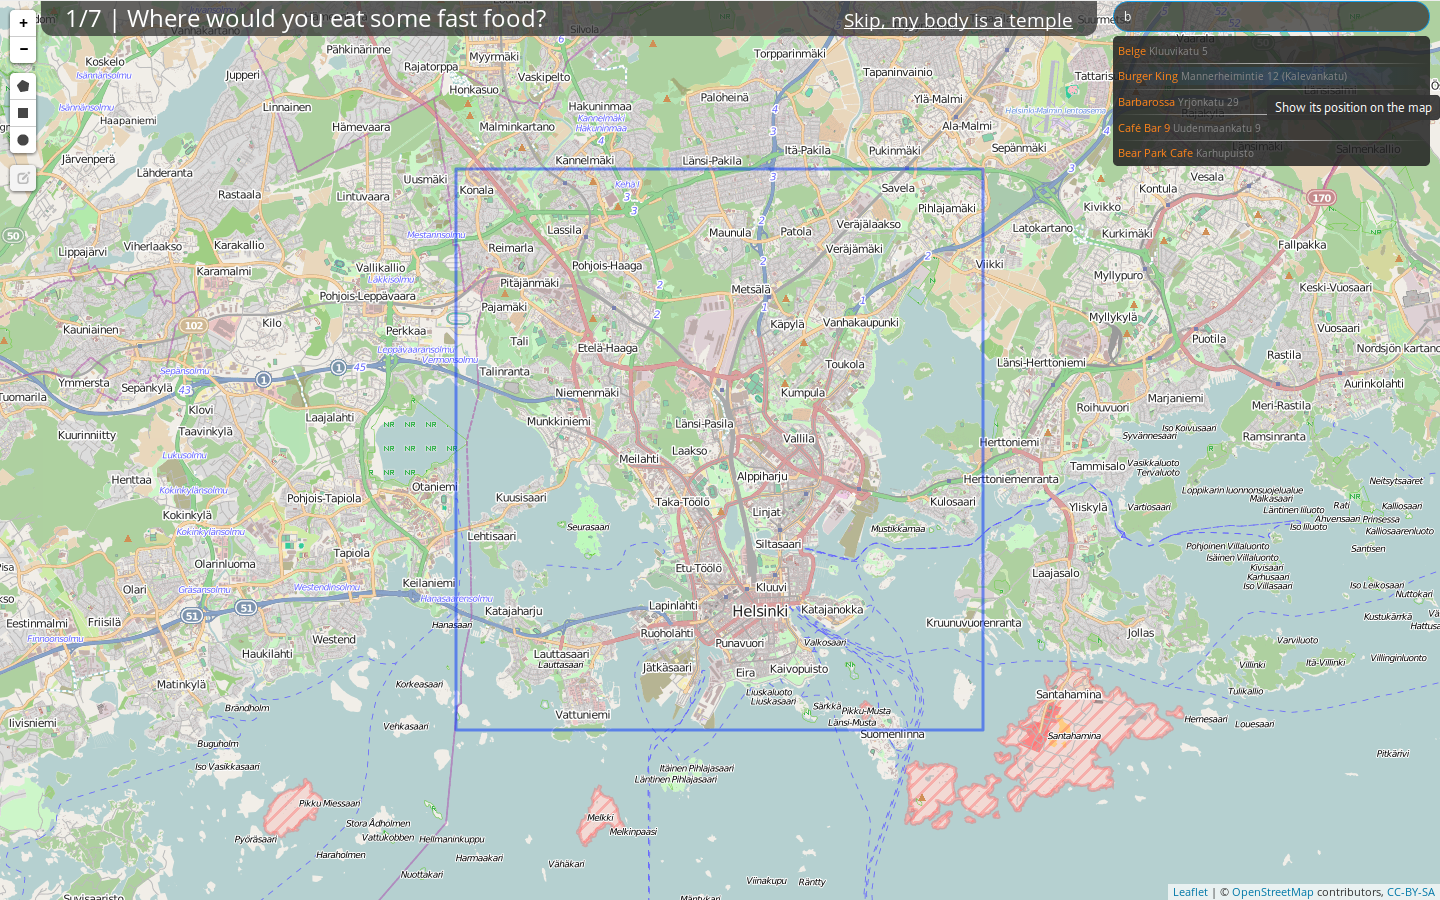
\includegraphics[width=\textwidth]{survey}
        \caption{The main screen of the survey.}
    \end{subfigure}

    \begin{subfigure}[b]{\textwidth}
        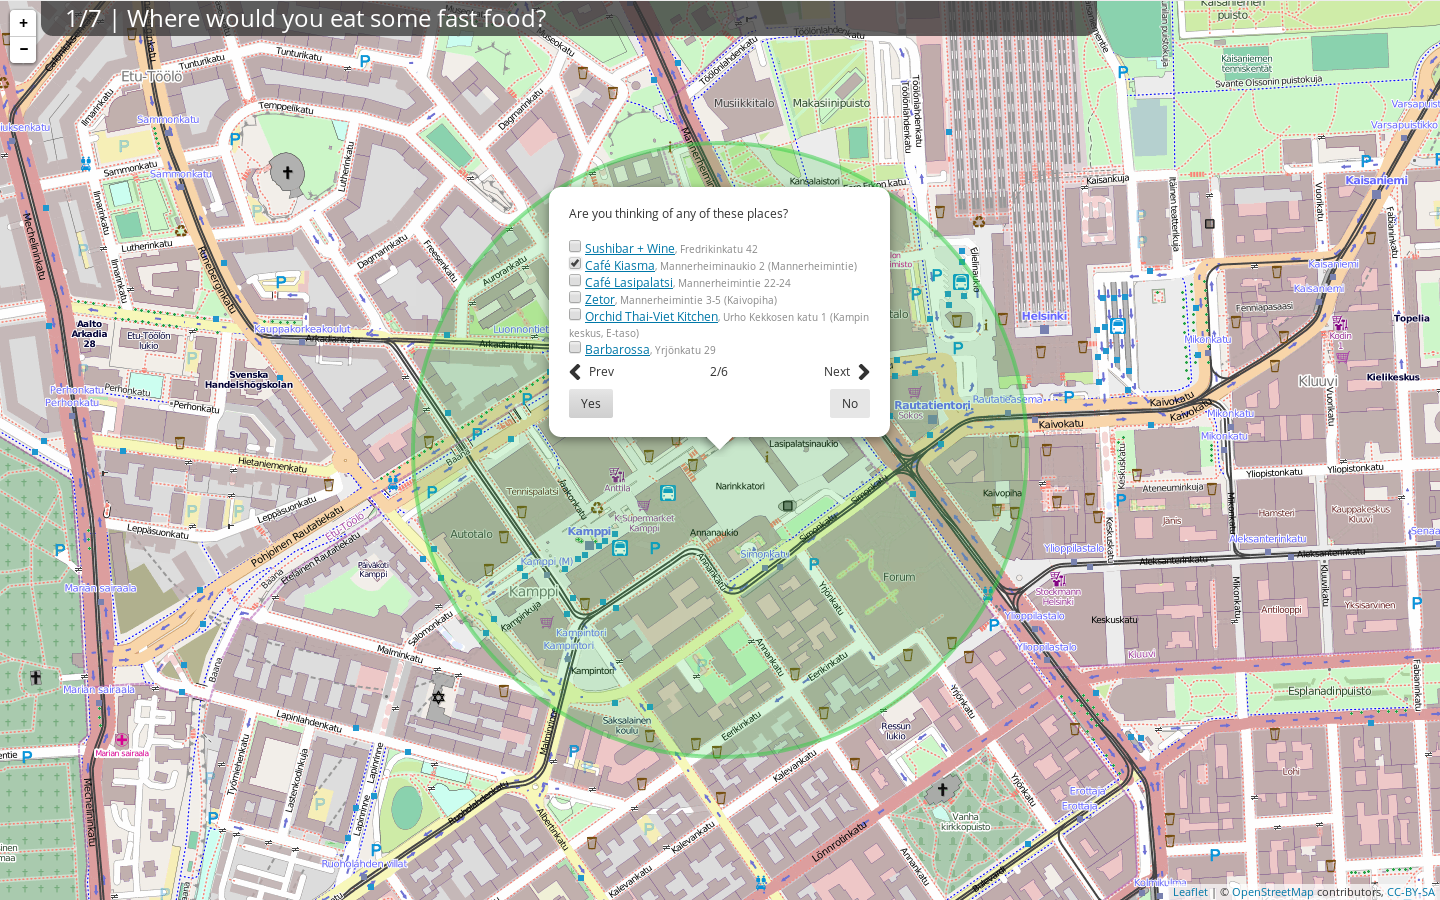
\includegraphics[width=\textwidth]{survey_venues}
        \caption{After an area have been drawn, the answer can be refined by
        choosing relevant venues from the dataset.}
    \end{subfigure}
    \caption{Website survey interface.\label{fig:survey}}
\end{figure}

\begin{comments}
number of answers, analysis of the results(?).
Rather tell about the slifht modification to ask directly for neighborhood
similar to those in Paris.
\end{comments}

\begin{table}[ht]
    \centering
    \begin{tabularx}{\textwidth}{lXX}
        \toprule
	Name & Question label & Relevant categories \\
        \midrule
	\texttt{fastfood} & Where would you eat some fast food?                       & Food \\
	\texttt{romance}  & Where would you bring your date to a romantic restaurant? & Food \\
	\texttt{coffee}   & Where would you drink a cozy coffee?                      & Tea Room, Bistro, Café, Coffee Shop, Cafeteria \\
	\texttt{clothes}  & Where would you buy new fancy clothes?                    & Clothing Store, Department Store, Fabric Shop, Flea Market, Mall \\
	\texttt{party}    & Where would you hangout with your friends?                & Nightlife Spot \\
	\texttt{sport}    & Where would you go to run in nature?                      &  Outdoors \& Recreation \\
	\texttt{culture}  & Where would you enjoy some cultural attractions?          & Art Gallery, Comedy Club, Concert Hall, Country Dance Club, Historic Site, Museum, Movie Theater, Music Venue, Outdoor Sculpture, Performing Arts Venue, Public Art, Street Art \\
        \bottomrule
    \end{tabularx}
    \caption[Question list]{The seven questions asked to gather human
    input.\label{tab:questions}}
\end{table}

\section{Exploration}

While collecting these data, it was helpful to explore them, in order to
discover features that could characterize places and help cluster them into
similar groups.

\subsection{Time}

The time at which check-ins occur is undoubtedly a important variable. For
instance, \textcite{UrbanStory12} performed topic modelling from the text of
check-in tweets and showed that various topics exhibit daily or weekly
patterns. Likewise, \textcite{TimeCluster13} clustered cells of a rectangular
grid according to their repartition of check-ins over categories and time of
day.

Thus we first looked at when check-ins are performed, and how it differed from
city to city \autoref{fig:time_checkin}. Then we adopted a venue-centric view
and clustered locations according to which time they are active
\autoref{fig:day_cluster}, which also depend of the city
\autoref{fig:time_cluster_size}.

\begin{figure}[hbt]
    \begin{subfigure}[b]{\textwidth}
    \centering
    \iftoggle{EXTERNALPGF}{%
        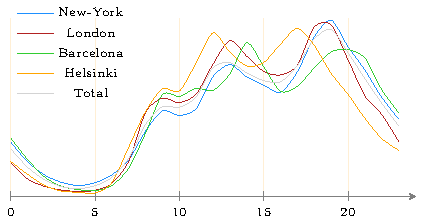
\includegraphics[width=\textwidth]{daily_checkin}
    }{%
        \input{mkfigs/daily_checkin}
    }
    \caption[Pattern of check-in during the day]{Generally, the activity is at
    its lowest around 5 \am{}\ and during the day, there are three peaks: one
when people go to work in the morning, one in the middle of the day and the
last one at the end of the evening. Yet, depending of the city, these peaks do
not happen at the same time, nor with the same intensity.
\label{fig:daily_checkin}}
    \end{subfigure}

    \begin{subfigure}[b]{\textwidth}
    \centering
    \iftoggle{EXTERNALPGF}{%
        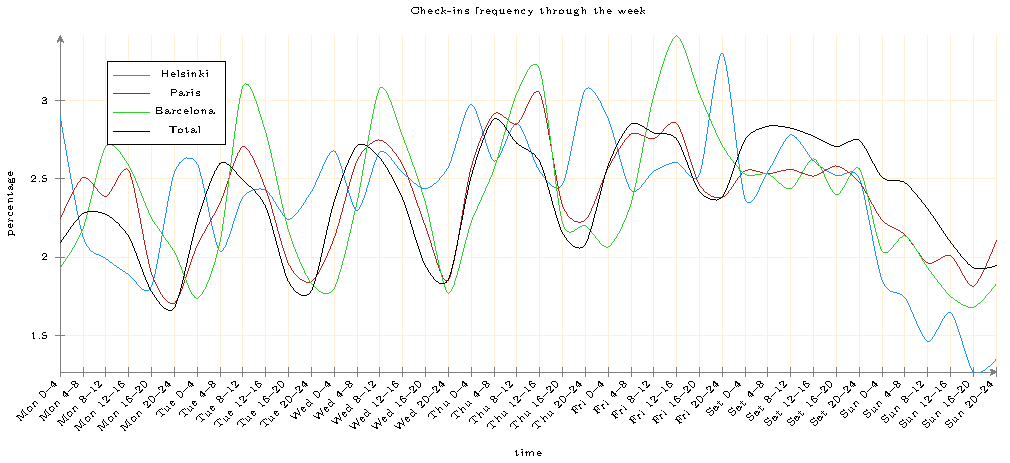
\includegraphics[width=\textwidth]{weekly_checkin}
    }{%
        \input{mkfigs/weekly_checkin}
    }
    \caption[Pattern of check-in during the week]{During the week, patterns
        are less clear.  \label{fig:weekly_checkin}}
    \end{subfigure}
    \caption{Check-ins temporal pattern.\label{fig:time_checkin}}
\end{figure}

\begin{figure}[hbt]
    \begin{subfigure}[b]{\textwidth}
    \centering
    \iftoggle{EXTERNALPGF}{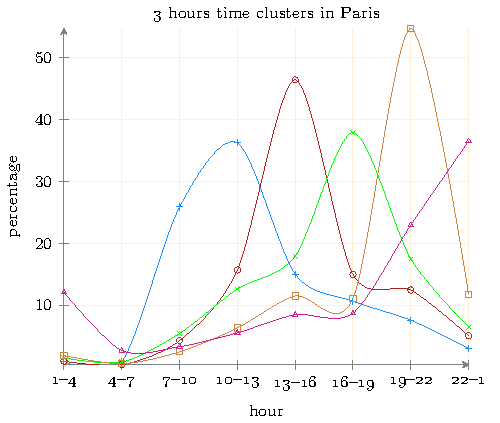
\includegraphics[width=\textwidth]{day_cluster_3h}}{\input{mkfigs/day_cluster_3h}}
    \end{subfigure}

    \begin{subfigure}[b]{\textwidth}
    \centering
    \iftoggle{EXTERNALPGF}{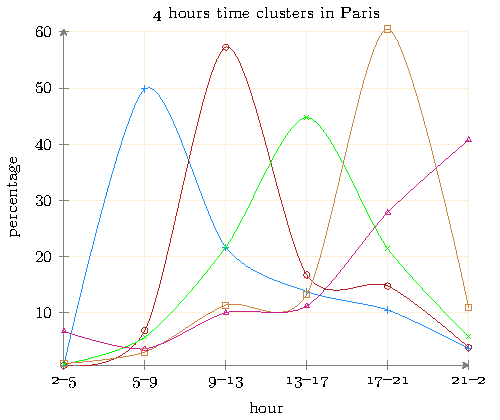
\includegraphics[width=\textwidth]{day_cluster_4h}}{\input{mkfigs/day_cluster_4h}}
    \end{subfigure}
    \caption[Venues clustered by time of check-ins]{Venues clustered by time
    of check-ins. \label{fig:day_cluster}}
\end{figure}

\newgeometry{left=0.3cm,right=0.3cm,bottom=0.1cm,top=0.1cm}
\begin{center}
\begin{figure}[hbt]
    \begin{subfigure}[b]{0.4\textwidth}
    \centering
    \iftoggle{EXTERNALPGF}{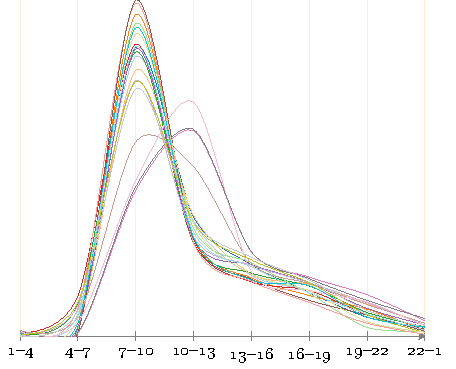
\includegraphics[height=0.18\textheight]{cluster_day_3h_cl1}}{\input{mkfigs/cluster_day_3h_cl1}}
    \end{subfigure}~
    \begin{subfigure}[b]{0.4\textwidth}
    \centering
    \iftoggle{EXTERNALPGF}{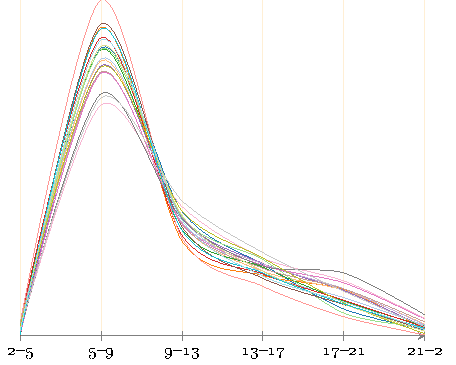
\includegraphics[height=0.18\textheight]{cluster_day_4h_cl1}}{\input{mkfigs/cluster_day_4h_cl1}}
    \end{subfigure}

    \begin{subfigure}[b]{0.4\textwidth}
    \centering
    \iftoggle{EXTERNALPGF}{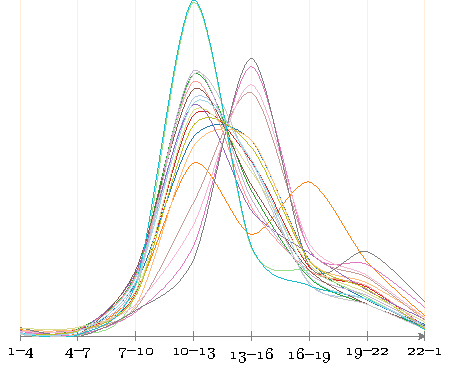
\includegraphics[height=0.18\textheight]{cluster_day_3h_cl2}}{\input{mkfigs/cluster_day_3h_cl2}}
    \end{subfigure}~
    \begin{subfigure}[b]{0.4\textwidth}
    \centering
    \iftoggle{EXTERNALPGF}{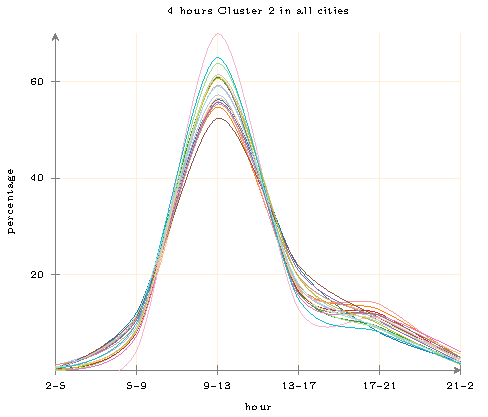
\includegraphics[height=0.18\textheight]{cluster_day_4h_cl2}}{\input{mkfigs/cluster_day_4h_cl2}}
    \end{subfigure}

    \begin{subfigure}[b]{0.4\textwidth}
    \centering
    \iftoggle{EXTERNALPGF}{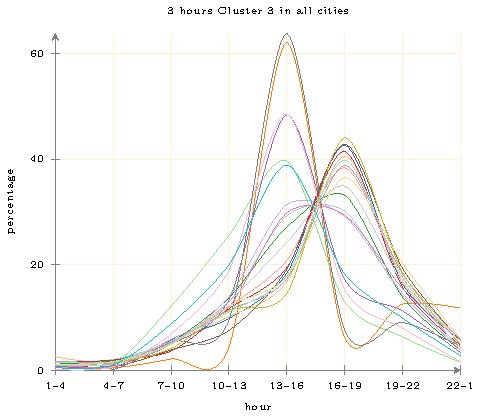
\includegraphics[height=0.18\textheight]{cluster_day_3h_cl3}}{\input{mkfigs/cluster_day_3h_cl3}}
    \end{subfigure}~
    \begin{subfigure}[b]{0.4\textwidth}
    \centering
    \iftoggle{EXTERNALPGF}{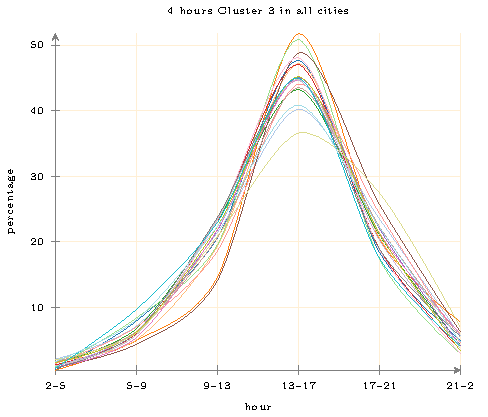
\includegraphics[height=0.18\textheight]{cluster_day_4h_cl3}}{\input{mkfigs/cluster_day_4h_cl3}}
    \end{subfigure}

    \begin{subfigure}[b]{0.4\textwidth}
    \centering
    \iftoggle{EXTERNALPGF}{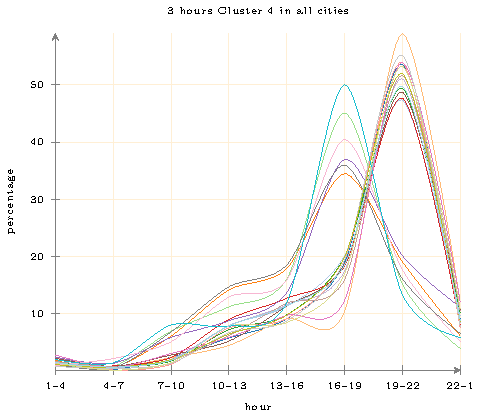
\includegraphics[height=0.18\textheight]{cluster_day_3h_cl4}}{\input{mkfigs/cluster_day_3h_cl4}}
    \end{subfigure}~
    \begin{subfigure}[b]{0.4\textwidth}
    \centering
    \iftoggle{EXTERNALPGF}{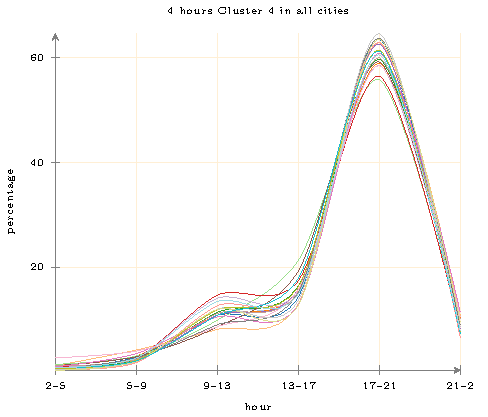
\includegraphics[height=0.18\textheight]{cluster_day_4h_cl4}}{\input{mkfigs/cluster_day_4h_cl4}}
    \end{subfigure}

    \begin{subfigure}[b]{0.4\textwidth}
    \centering
    \iftoggle{EXTERNALPGF}{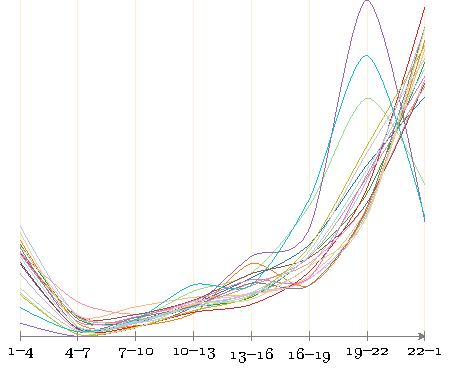
\includegraphics[height=0.18\textheight]{cluster_day_3h_cl5}}{\input{mkfigs/cluster_day_3h_cl5}}
    \end{subfigure}~
    \begin{subfigure}[b]{0.4\textwidth}
    \centering
    \iftoggle{EXTERNALPGF}{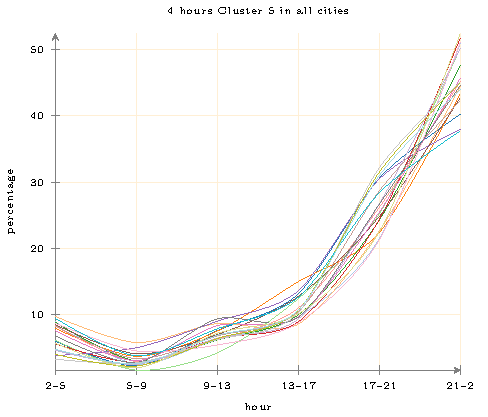
\includegraphics[height=0.18\textheight]{cluster_day_4h_cl5}}{\input{mkfigs/cluster_day_4h_cl5}}
    \end{subfigure}
    \caption[Venues cluster by time among all the cities]{4 hours time
    clusters are the same among all cities, whereas it is not the case for 3
hours clusters. \label{fig:time_cluster_size}}
\end{figure}
\end{center}
\restoregeometry

\subsection{Space}

The other main characteristic of every check-in is where it takes place. We
focus on two spatial feature of venues. First, was does the surrounding looks
like in terms of categories. For instance, if a restaurant is mainly
surrounded by night life places and another by education buildings, they
probably have different customers. Second, venues are not uniformly
distributed within the city and the density of nearby locations is a
discriminative feature as well. For instance in \autoref{fig:density_paris},
we can clearly distinguish venues belonging to the city center from the
others.

\begin{figure}[hbtp]
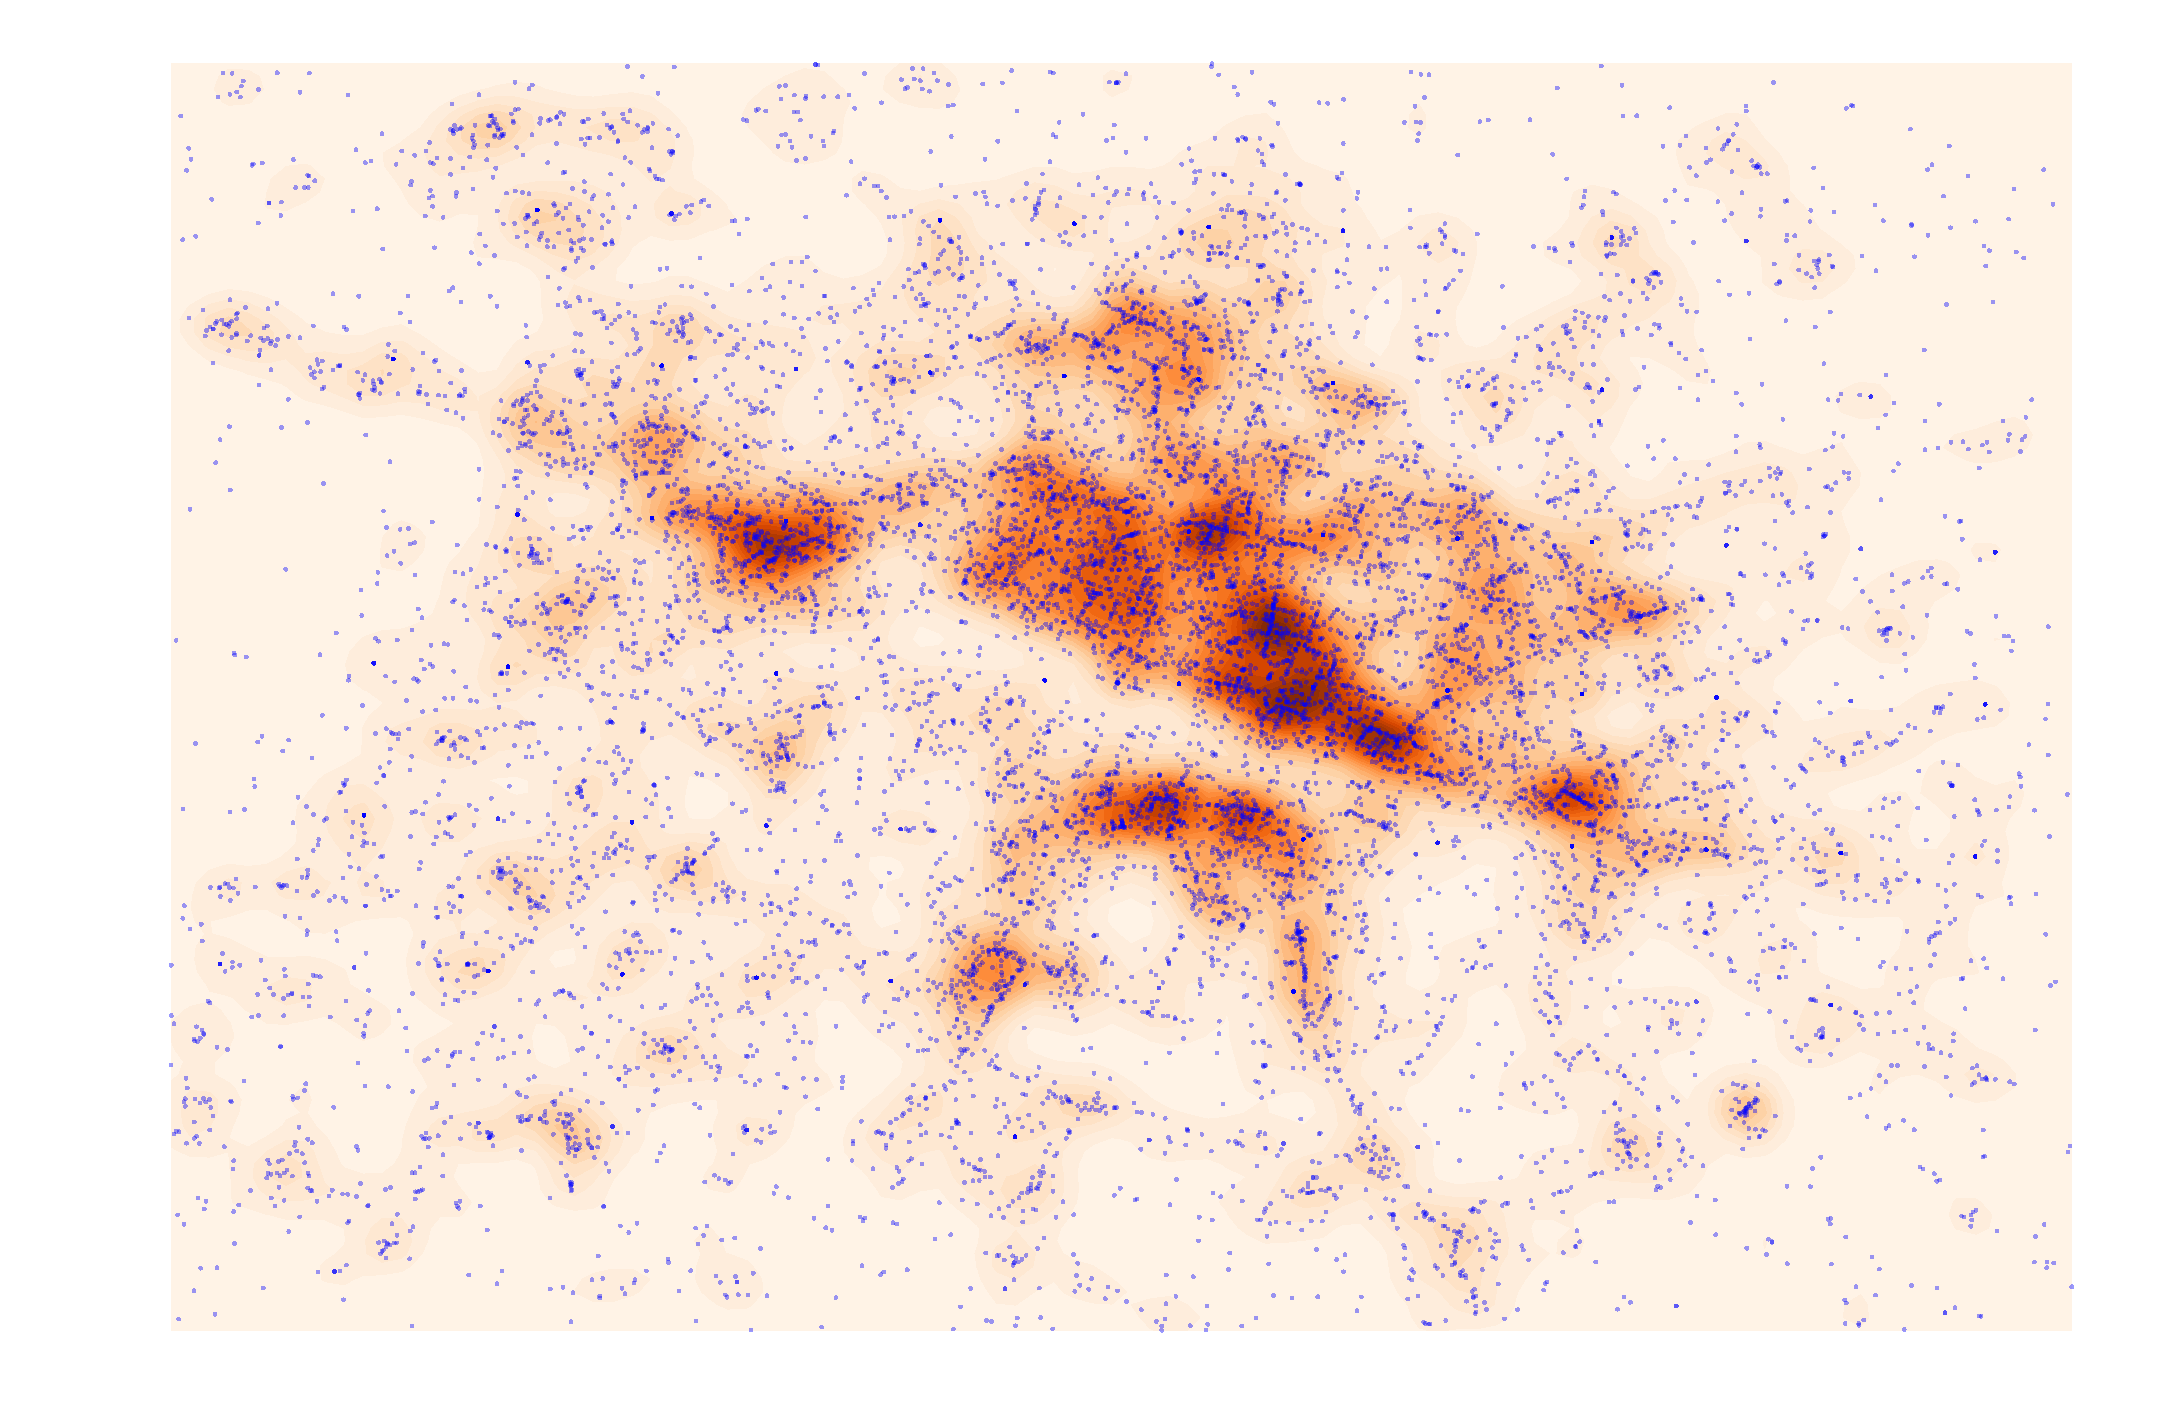
\includegraphics[width=\textwidth]{density_paris_venues}
\caption[Venue density in Paris]{Estimated venues density in Paris by a
	Gaussian kernel.\label{fig:density_paris}}
\end{figure}

\subsection{Location entropy}

\Textcite{Entropy10} showed that \enquote{location entropy, which measures the
diversity of unique visitors of a location} gives good indication of the
sociability level of venues and therefore help predicting friendship ties within
\gls{lbsn}.

Let $\mathcal{U}$ be the set of users and $\mathcal{V}$ the one of venues. For
each venue $v \in \mathcal{V}$, we can gather the set of check-ins $c_v$ that
occurred there as well as the corresponding users $[u_1, u_2, u_2, \ldots,
u_n]$ (note that the same users can check-in multiple times). Then we
transform this list to a frequency distribution $f_v$ over $\mathcal{U}$ and
compute the normalized entropy: \[
    H(v) = -\frac{1}{\log\left(\left| \mathcal{U}\right|\right)}
\sum_{u\in \mathcal{U}} f_v(u) \log(f_v(u)) \]

Show examples with high and low value in Paris and Barcelona:

\begin{tabular}{llr}
	\toprule
	Name                    & Category            & Entropy \\
	\midrule
    Castellers de Barcelona       & Non-Profit        & 0.0139 \\
    Café de la Pompeu             & Café              & 0.0172 \\
    Ràdio 4                       & Radio Station     & 0.0176 \\
    La Comarca                    & Home (private)    & 0.0180 \\
    House castellar               & Home (private)    & 0.0181 \\
    Av Tomas Gimenez              & Bar               & 0.0186 \\
    Torre De Barad-Dur            & Building          & 0.0192 \\
    \midrule
    Blue Acacia                   & Office            & 0.0119 \\
    Boutique Orange               & Electronics Store & 0.0141 \\
    Regus                         & Office            & 0.0163 \\
    Café Pierre                   & French Restaurant & 0.0181 \\
    my home 2                     & Home (private)    & 0.0193 \\
    10e arrondissement – Entrepôt & \& Municipalities & 0.0213 \\
    Scanblog                      & Office            & 0.0221 \\
	\midrule
    Parc de la Ciutadella          & Park                & 0.5188 \\
    Apple Store                    & Electronics Store   & 0.5358 \\
    Parc Güell                     & Park                & 0.5666 \\
    Plaça de Catalunya             & Plaza               & 0.5835 \\
    Sants Estació                  & Train Station       & 0.6298 \\
    Sagrada Família                & Government Building & 0.6309 \\
    Camp Nou                       & Stadium             & 0.6852 \\
    \midrule
    Arc de Triomphe                & Government Building & 0.5831 \\
    Cathédrale Notre-Dame de Paris & Spiritual Center    & 0.5874 \\
    Gare SNCF Paris Montparnasse   & Train Station       & 0.6141 \\
    Musée du Louvre                & Museum              & 0.6444 \\
    Gare SNCF Gare de Lyon         & Train Station       & 0.6460 \\
    Tour Eiffel                    & Government Building & 0.6618 \\
    Gare SNCF Paris Nord           & Train Station       & 0.6707 \\
	\bottomrule
\end{tabular}

Following the same idea, we also computed the entropy of locations with
respect to time of check-ins. Indeed, it distinguishes between a railway
station active all day along and a restaurant only open during lunch hours.
We are also expecting a link between the two entropies, as place that stay
open longer have more chance to be enjoy a various crowd. But it is not the
cases on \autoref{fig:two_entropies}, as some places are visited all the time
by a very small group of people

\begin{figure}[hbtp]
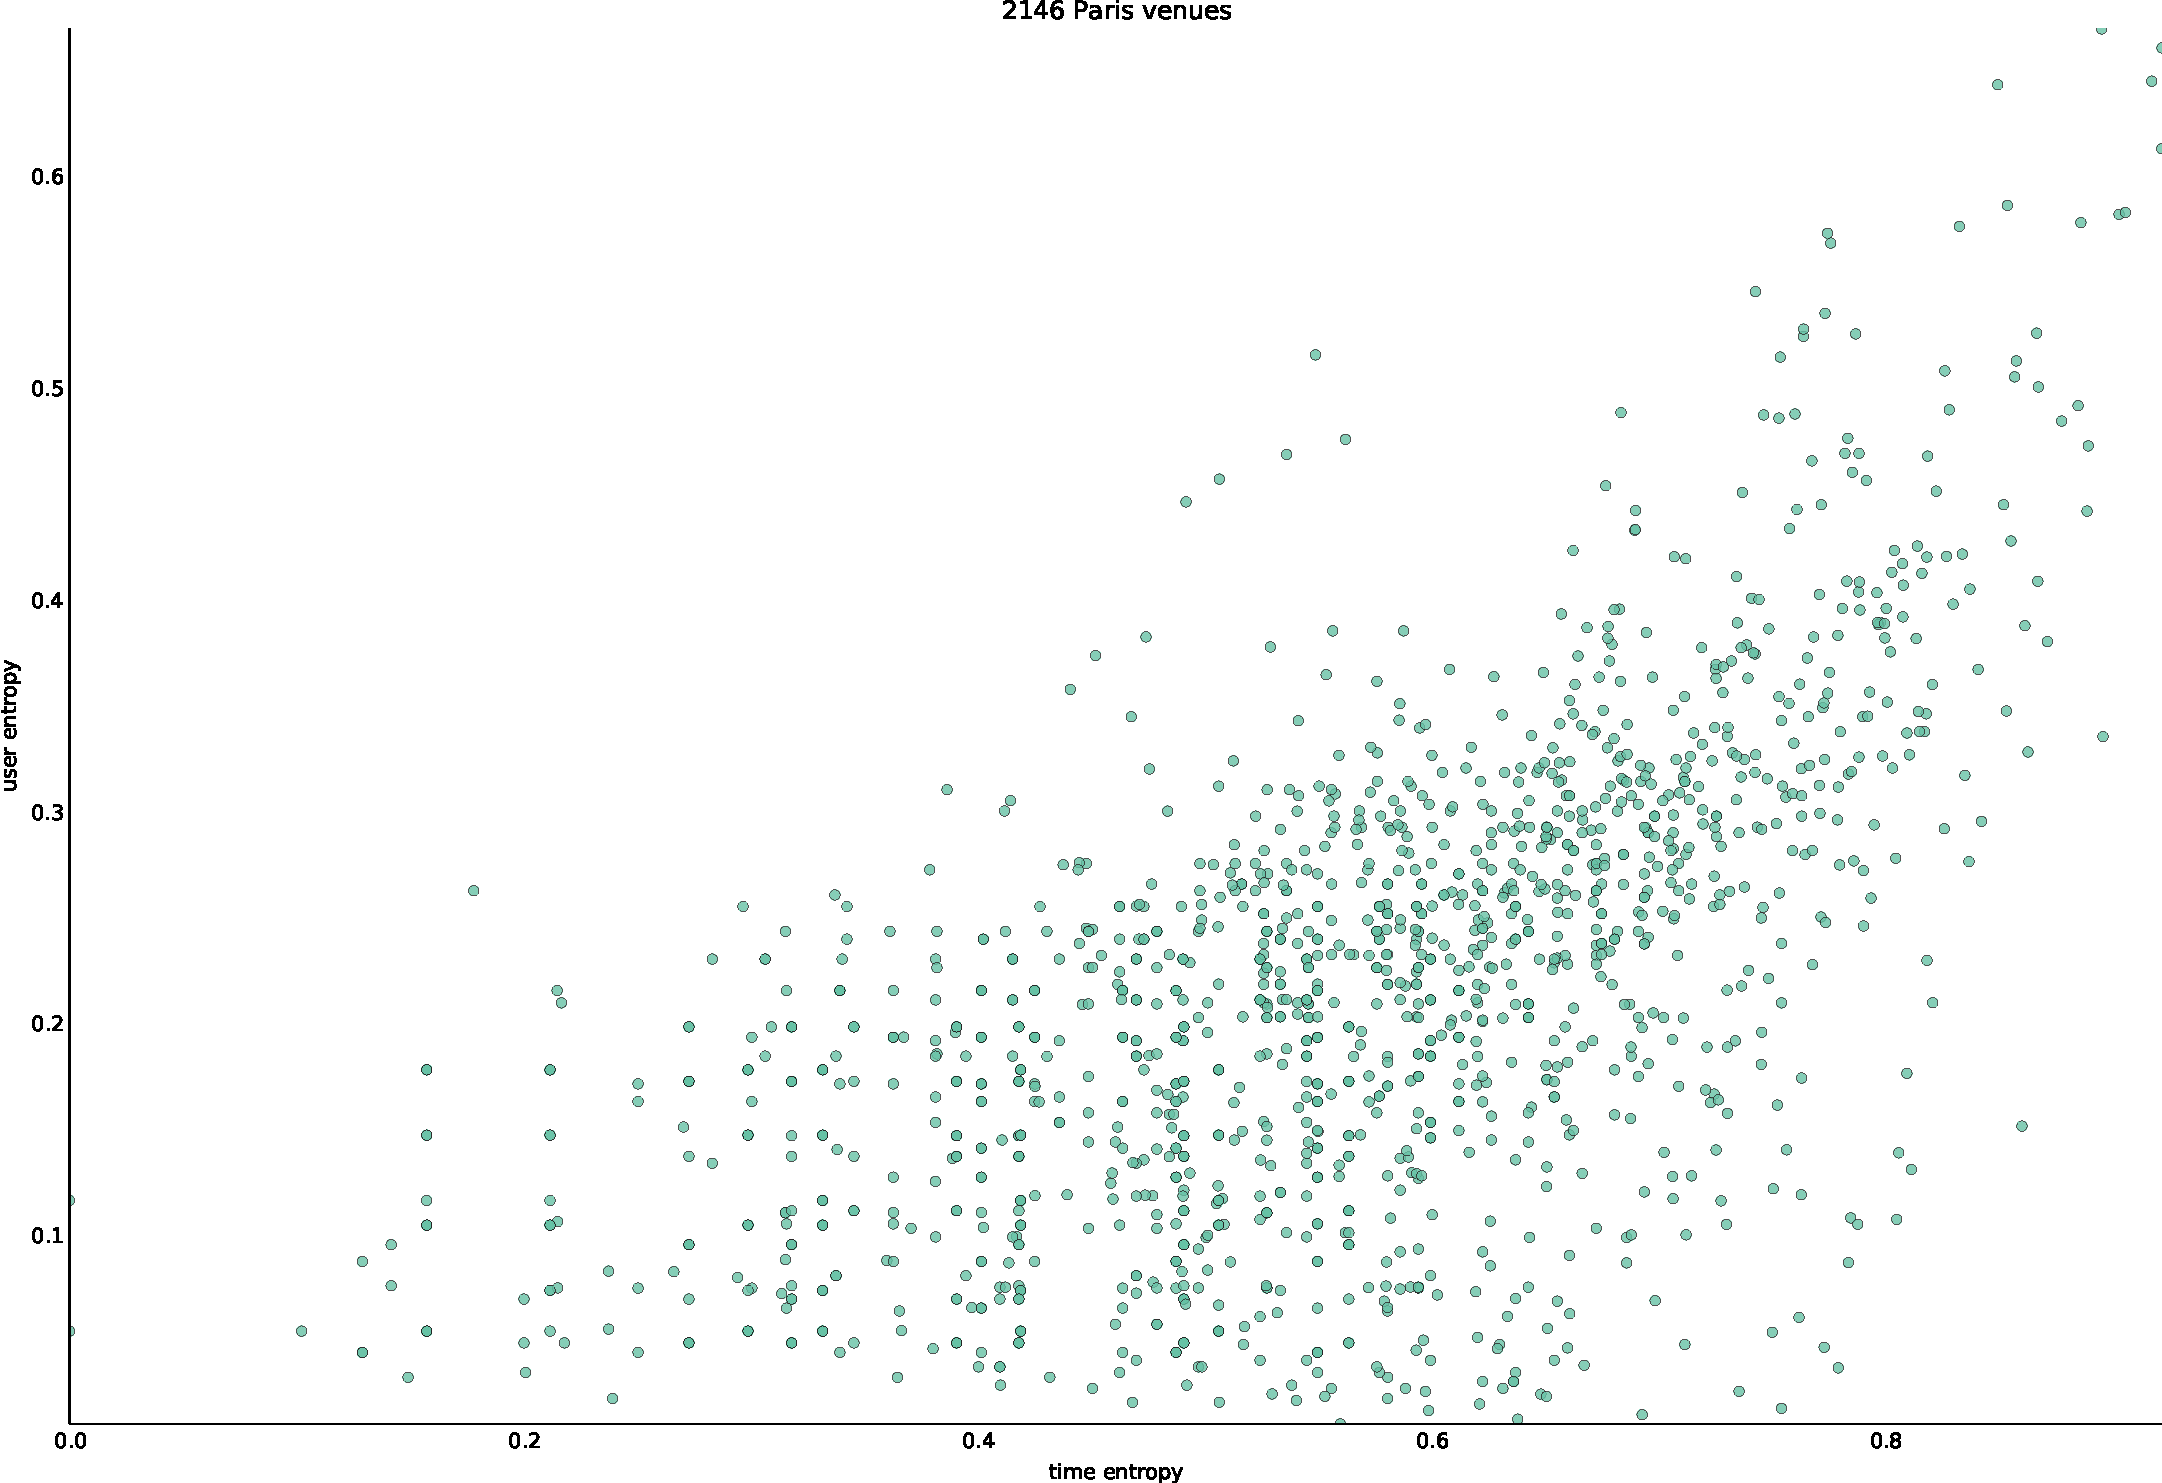
\includegraphics[width=\textwidth]{two_entropies}
\caption{Venues entropy with respect to user population and time of check-in
during the day. \label{fig:two_entropies}}
\end{figure}


\subsection{Photos}

Assume that photos are background signal of interest within city. Use exact
grid algo from \autocite{Agarwal2006spatial} to compute discrepancy with
check-ins measurement (and conversely). \marginpar{give real examples} More
photos in touristic places, more check-in in “event” places (railway, stadium)

Look at high and low focus places: not so interesting either. High value are
for popular places like park or monument whereas low (but not zero) are for
mundane place (like pizzeria) close to famous locations.

\section{Chosen representation}

Based on the insights gained by exploring the dataset, we settle to represents
each venues by the numerical vector presented in \autoref{tab:venuefeatures}.
The features involving the surrounding (numbered from 6 to 16 and 25 to 30)
were weighted by a 2D Gaussian of radius $r=350$ meters.

\begin{table}[hb]
    \centering
    \begin{tabularx}{\textwidth}{lX}
        \toprule
        index & description \\
        \midrule
	\datasetRow{}0 & Number of likes \\
	\datasetRow{}1 & Number of unique users \\
	\datasetRow{}2 & Number of total check-ins \\
        3 & User entropy \\
        4 & Venue density \\
	\datasetRow{}5 & Venue top level category \\
        6 & \enquote{Arts \& Entertainment} venues around \\
        7 & \enquote{College \& University} venues around \\
        8 & \enquote{Food} venues around \\
        9 & \enquote{Nightlife Spot} venues around \\
        10 & \enquote{Outdoors \& Recreation} venues around \\
        11 & \enquote{Shop \& Service} venues around \\
        12 & \enquote{Professional \& Other Places} venues around \\
        13 & \enquote{Residence} venues around \\
        14 & \enquote{Travel \& Transport} venues around \\
	15 & Ratio of photos over check-ins \\
	16 & Ratio of photos associated to the venue over photos linked to other venues \\
	17 & More than half of the check-ins occurs during the week-end \\
	18 & Frequency of check-ins between 2 \am{} and 6 \am{} \\
	19 & Frequency of check-ins between 6 \am{} and 10 \am{} \\
	20 & Frequency of check-ins between 10 \am{} and 2 \hpm{} \\
	21 & Frequency of check-ins between 2 \hpm{} and 6 \hpm{} \\
	22 & Frequency of check-ins between 6 \hpm{} and 10 \hpm{} \\
	23 & Frequency of check-ins between 10 \hpm{} and 2 \am{} \\
	24 & Time entropy \\
	25 & Frequency of neighbouring check-ins between 2 \am{} and 6 \am{} \\
	26 & Frequency of neighbouring check-ins between 6 \am{} and 10 \am{} \\
	27 & Frequency of neighbouring check-ins between 10 \am{} and 2 \hpm{} \\
	28 & Frequency of neighbouring check-ins between 2 \hpm{} and 6 \hpm{} \\
	29 & Frequency of neighbouring check-ins between 6 \hpm{} and 10 \hpm{} \\
	30 & Frequency of neighbouring check-ins between 10 \hpm{} and 2 \am{} \\
        \bottomrule
    \end{tabularx}
    \caption[Venue features]{Feature representation of Foursquare venues,
	    taking surrounding into account. \colorbox{Moccasin}{Shaded
	    features} are provided directly by Foursquare database whereas the
	    others were computed solely based on the partial information
	    contained in the dataset.\label{tab:venuefeatures}}
\end{table}


% \chapter{Methods}
\label{chap:methods}

\section{Closest Neighbors}

\subsection{Dimensionality reduction}

\begin{flushright}{\slshape
	If people could see in high dimensions \\
	machine learning would not be necessary.
} \\ \medskip
--- Pedro \Textcite{MLKnowledge12}
\end{flushright}

So far, t-Distributed Stochastic Neighbor Embedding \autocite{tSNE08} seems
the most promising method.

\subsection{Metric learning}

After reading some surveys \autocite{MetricSurvey06, MetricSurvey13}, I tried
Information-theoretic Metric Learning \autocite{InfoMetric07} and
Gradient-Boosted Largest Margin Nearest Neighbors \autocite{GBLMNN12} although
it would be interesting to also use histogram distance
\autocite{HistogramDistance02}

\section{Matching under constraint}

\section{Visualization}

% \chapter{Results}
\label{chap:result}

% \chapter{Related work}
\label{chap:related}

Our work can be related to several lines of research within the field of urban
computing. First, mining spatial data (photos, check-ins, and GPS
trajectories) to find places and their semantics, which is a potential
application of the broad term of \enquote{smart city} and has very concrete
implications for major websites. This task also remains of topic modeling,
with more constraints regarding space and time. After finding places, we want
to learn metrics to compare them in a meaningful and accurate way.

\paragraph{photos}

Such places are usually defined by their density, and thus one seeks to find
high concentration of people taking photos there. For instance,
\textcite{Deng2009} use \textsc{DBSCAN} to cluster Flickr photos and then look
at tags co occurrence within clusters to identify their meaning.
\Textcite{Rattenbury2009} also employ various spatial methods to discover
regions in San Francisco where one photo tag appears in burst. The shape of
these hotspot regions can be refined by looking at the orientation of each
photo \autocite{Hotspots12}. Another way of identify hotspots is second order
Ripley's K-function \autocite{TagHotspot12}. Basically, it is a statistical
test for the hypothesis that points are distributed according to a Poisson
process. It indicates how they \enquote{interact with each other, either
\enquote{repulsively} [\dots] or \enquote{attractively}.} Furthermore, it is
able to process regions with varying density of pictures. Besides location
finding, analyzing photos can also lead to other applications, like
recommending routes for tourists based on a graph of points of interest
\autocite{CityItineraries10} and even ensure that these paths are as agreeable
as possible \autocite{Quercia2014}.

\paragraph{check-ins}

Moving from Flickr to \glspl{lbsn} allows searching for larger areas like
neighborhoods. \Textcite{SocioMap12} collect general tweets and perform
sentiment analysis as well as movement detection to draw a socio cognitive map
of the Kinki region in Japan which helps user to make decision regarding where
to live. Closer to our work, \textcite{Livehoods12} analyse 18 millions
check-ins to find so-called
\emph{Livehoods}\footnote{\href{http://livehoods.org/}{\url{livehoods.org}}}.
They build a $m$ spatial neighbors graph of venues with edges weighted by the
cosine similarity between their user distribution and then perform spectral
clustering. Faced with the same difficulty as ours to evaluate their results,
they interview residents of Pittsburgh who validate the obtained subdivisions.
Another approach was proposed by
\textcite{Hoodsquare13}\footnote{\href{http://pizza.cl.cam.ac.uk/hoodsquare/}%
{\url{hoodsquare.org}}}, also based on Foursquare check-ins. Each venue is
described by its category, its peak time activity and a binary label:
touristic or not. They are clustered in hotspots along each of these dimensions
by the \textsc{OPTICS} algorithm. The city is then divided into a regular grid
and cells are described by their hotspot density for each feature.
\marginpar{Mention evaluation using tweets mention?} Finally, similar cells
are clustered into neighborhoods. The main difference between this last two
works and ours is that they do not explicitly mention distance between the
neighborhoods they recover.

\paragraph{GPS}

In addition to static data like photos, another line of work takes advantage
of the dynamic nature of human movement to mine trajectories. For instance,
\textcite{MAtlas11} analyze GPS data in Italian cities to find temporal
patterns, which can then be used for event detection or traffic jam
regulation. Similarly, \textcite{GPSStay10} extract stay points from car GPS
data and assess their significance by how many visitors go there, how far they
traveled to reach them and how long they stay. \Textcite{TrajROI11} describe
efficient techniques to perform closely related tasks. Once the semantics of
locations is known, it is still challenging to find frequent patterns
efficiently \autocite{SemanticTrajectories14}. Interested reader will find
more information in a recent survey \autocite{TrajSurvey13}.


\paragraph{Industrial applications}

The problem of identifying and characterizing neighborhoods has also been
addressed by companies. For instance, research in \flickr{} has shown that by
computing the $\alpha$-shape of a set of tagged photos (which is a
generalisation of its convex hull \autocite{AlphaShape83}) one can recover
boundaries of
neighborhoods\footnote{\href{http://code.flickr.net/2008/10/30/the-shape-of-alpha/}%
{\url{code.flickr.net/2008/10/30/the-shape-of-alpha}}}. Likewise, Airbnb, a
social lodging renting website, has accumulated a lot of spatial data as well
as textual reviews, which can be used to rank cities by hospitality
\footnote{\href{http://nerds.airbnb.com/most-hospitable-cities/}%
{\url{nerds.airbnb.com/most-hospitable-cities}}} as well as discovering
neighborhoods
\footnote{\href{https://www.airbnb.com/locations}{\url{airbnb.com/locations}}}.
However, the methods and details of these commercial systems are not publicly
available. Finally, engineers at \fs{} used 1.5 billion check-ins to compare
activities of different part of cities in
US\footnote{\href{http://engineering.foursquare.com/2012/03/08/a-hackday-project-what-neighborhood-is-the}%
{\url{engineering.foursquare.com/2012/03/08/a}}}.

\paragraph{Spatio-temporal topic modeling}

Finding such places can also be thought as trying \enquote{to discover the
hidden thematic structure in large archives of documents}, which is the
definition of probabilistic topic modeling according to \textcite{topicModel}.
Usually such documents are textual and can be combined in any way to form a
theme. Here we do not necessarily have text (although photos tags and check-ins
contain some) but we have additional spatio-temporal constraints for
neighborhoods (or topic) to be localized. For instance,
\textcite{GeoTopicYin11} fix a number $K$ of localized topics to be discovered,
as well as a set of $N$ weighted Gaussian spatial regions. Then they apply
their Latent Geographical Topic Analysis framework: each region has a topic
distribution and each topic is a multinomial distribution over all possible
photos tags. The parameters of the model are learned by an EM algorithm. By
taking user into account, this approach provides recommendations
\autocite{GeoTopicKurashima2013}. The same can be done for localized tweets
with a hierarchical model of topics \autocite{nestedChinese13}. Recently,
precision and running time of such methods were improved by
\textcite{NonGaussianTopicKling14}. Finally, some topics are localized in time
as well as in space (like \texttt{earthquake}) and this calls for more specific
methods. \Textcite{TwitterBurst13} extract keywords from twitter in a moving
sliding windows and keep those that are bursty. Using localized tweets, they
estimate the topic spatial distribution but because of sparsity and noise, it
requires a regularisation based on a co occurrences and identification of
anchor keywords. A scalable online approximate solution is described in
\autocite{GeoScope}.

\paragraph{Smart cities}

Smart cities in general are a new area which offers a lot of scientific
challenges \autocite[Chapter 4]{Eunoia13} as well as potential benefits in
terms of sustainability and well being by making use of Information
Technologies \autocite{SmartCities13}. How IBM was able to tap into Helsinki
open data to provide a compelling narrative of citizens' engagement and promote
the World Design Capital event in 2012 \autocite{HelsinkiSCC11}.

% (or playable cities: \url{http://www.watershed.co.uk/playablecity/overview/},
% \ie{} avoid focusing solely on monetization:
% \url{http://radar.oreilly.com/2014/05/most-of-what-we-need-for-smart-cities-already-exists.html})

\paragraph{Metric learning}

Some pointers we already given in \autoref{sec:metric} but the topic is
abundant. For instance, learning a Mahalanobis distance was introduced more
than ten years ago \autocite{Xing2002}. Later, the optimization problem was
given a simpler formulation, which has therefore a lower complexity
\autocite{Shen2011}. Two recent works are more sophisticated and use two-stage
statistical approach \autocite{Wang2014} and sparse local metrics
\autocite{SparseMetric14}.

\iffalse
\paragraph{Matching and multiple domains}

\begin{comments}
	So far, I haven't really found a connection between these papers and my work
	so I will probably remove them.
	\begin{itemize}
		\item 2 domains with the same number of objects in each (but described
			by different features) \autocite{Klami2013}.
		\item many to many matching from arbitrary number of domain and
			different number of object in each by using a common latent space
			\autocite{iwata2013unsupervised}
		\item Give unknown $K$ sources of observations and their pairwise
			dissimilarity, find the optimal set of sources to learn a model
			for each one \autocite{Crammer2008}.
		\item Train a classifier in a source domain where there are a lot
			labeled examples and see how well it would perform on close target
			domain with less examples (and how to use those)
			\autocite{Ben-David2009}.
	\end{itemize}
\end{comments}
\fi

% \chapter{Conclusion}
\label{chap:conclusion}

% ********************************************************************
% Backmatter
%*******************************************************
\appendix
% \cleardoublepage
%%********************************************************************
% Appendix
%*******************************************************
% If problems with the headers: get headings in appendix etc. right
%\markboth{\spacedlowsmallcaps{Appendix}}{\spacedlowsmallcaps{Appendix}}
\chapter{Appendix Test}
\label{chap:appendix}
All this work was done on Linux, using many other open source tool such as
python, \LaTeX, firefox, …

%********************************************************************
% Other Stuff in the Back
%*******************************************************
% \cleardoublepage
% %********************************************************************
% Bibliography
%*******************************************************
% work-around to have small caps also here in the headline
\manualmark
\markboth{\spacedlowsmallcaps{\bibname}}{\spacedlowsmallcaps{\bibname}} % work-around to have small caps also
%\phantomsection 
\refstepcounter{dummy}
\addtocontents{toc}{\protect\vspace{\beforebibskip}} % to have the bib a bit from the rest in the toc
\addcontentsline{toc}{chapter}{\tocEntry{\bibname}}
\label{app:bibliography} 
% \bibliographystyle{plainnat}
% \bibliography{Bibliography}
\printbibliography{}

%\cleardoublepage\pagestyle{empty}

\hfill

\vfill


\pdfbookmark[0]{Colophon}{colophon}
\section*{Colophon}
This document was typeset using the typographical look-and-feel \texttt{classicthesis} developed by André Miede. 
The style was inspired by Robert Bringhurst's seminal book on typography ``\emph{The Elements of Typographic Style}''. 
\texttt{classicthesis} is available for both \LaTeX\ and \mLyX: 
\begin{center}
\url{http://code.google.com/p/classicthesis/}
\end{center}
Happy users of \texttt{classicthesis} usually send a real postcard to the author, a collection of postcards received so far is featured here: 
\begin{center}
\url{http://postcards.miede.de/}
\end{center}
 
\bigskip

% \noindent\finalVersionString


\end{document}
